\documentclass[a4paper,12pt]{report}

% --- Encoding & Font ---
\usepackage[utf8]{inputenc}
\usepackage[T5,T1]{fontenc}
\usepackage[english,vietnamese]{babel}
\usepackage{times}
\usepackage{lmodern}

% --- Page Layout ---
\usepackage[top=2.5cm, bottom=2.5cm, left=3cm, right=2.5cm]{geometry}
\usepackage{setspace}
\onehalfspacing

% --- Graphics ---
\usepackage{graphicx}
\usepackage{float}
\usepackage{subcaption}

% Pandoc image scaling & placement
\makeatletter
\def\maxwidth{\ifdim\Gin@nat@width>\linewidth\linewidth\else\Gin@nat@width\fi}
\def\maxheight{\ifdim\Gin@nat@height>\textheight\textheight\else\Gin@nat@height\fi}
\makeatother
\setkeys{Gin}{width=\maxwidth,height=\maxheight,keepaspectratio}
\makeatletter
\def\fps@figure{htbp}
\makeatother

% --- Tables ---
\usepackage{booktabs}
\usepackage{array}
\usepackage{longtable}
\usepackage{multirow}
\usepackage{tabularx}
\usepackage{calc}

% --- Math ---
\usepackage{amsmath}
\usepackage{amssymb}

% --- Code Listings & Verbatim with UTF-8 support ---
\usepackage{listings}
\usepackage{xcolor}
\usepackage{fancyvrb}
\usepackage{fvextra}

\definecolor{codebg}{RGB}{248,248,248}
\definecolor{codeframe}{RGB}{200,200,200}
\definecolor{codecomment}{RGB}{106,153,85}
\definecolor{codestring}{RGB}{163,21,21}
\definecolor{codekeyword}{RGB}{0,0,255}
\definecolor{ptitblue}{RGB}{0,51,153}

\lstdefinestyle{customstyle}{
  backgroundcolor=\color{codebg},
  frame=single,
  rulecolor=\color{codeframe},
  basicstyle=\ttfamily\footnotesize,
  keywordstyle=\color{codekeyword}\bfseries,
  commentstyle=\color{codecomment}\itshape,
  stringstyle=\color{codestring},
  showstringspaces=false,
  breaklines=true,
  tabsize=4,
  captionpos=b,
}
\lstset{style=customstyle}

\DefineVerbatimEnvironment{lstlisting}{Verbatim}{
  frame=single,
  rulecolor=\color{codeframe},
  fillcolor=\color{codebg},
  framesep=3mm,
  fontsize=\footnotesize,
  breaklines=true
}

% --- Hyperlinks ---
\usepackage[hidelinks]{hyperref}
\usepackage{url}
\usepackage{xurl}

% --- Section Formatting ---
\usepackage{titlesec}
\usepackage[titles]{tocloft}

% --- Compact TOC configuration to guarantee single-page fit ---
\setlength{\cftbeforetoctitleskip}{-15pt}
\setlength{\cftaftertoctitleskip}{15pt}
\setlength{\cftbeforechapskip}{4pt}
\setlength{\cftbeforesecskip}{1pt}

\titleformat{\chapter}[display]
  {\normalfont\fontsize{22}{26}\bfseries}
  {Chương \thechapter}{14pt}{\fontsize{22}{26}\bfseries}
\titlespacing*{\chapter}{0pt}{-10pt}{24pt}

\titleformat{\section}
  {\normalfont\fontsize{16}{20}\bfseries}{\thesection}{1em}{}
\titlespacing*{\section}{0pt}{18pt}{10pt}

\titleformat{\subsection}
  {\normalfont\fontsize{13}{17}\bfseries}{\thesubsection}{1em}{}
\titlespacing*{\subsection}{0pt}{14pt}{8pt}

\titleformat{\subsubsection}
  {\normalfont\fontsize{12}{15}\bfseries\itshape}{\thesubsubsection}{1em}{}
\titlespacing*{\subsubsection}{0pt}{10pt}{6pt}

% --- Caption ---
\usepackage{caption}
\captionsetup{font=small, labelfont=bf, skip=8pt}

% --- Header / Footer ---
\usepackage{fancyhdr}
\pagestyle{fancy}
\fancyhf{}
\fancyfoot[C]{\thepage}
\renewcommand{\headrulewidth}{0pt}

% --- TOC depth ---
\setcounter{tocdepth}{3}
\setcounter{secnumdepth}{3}

% --- Indentation ---
\usepackage{indentfirst}
\setlength{\parindent}{1cm}
\setlength{\emergencystretch}{3em}

% --- TikZ for cover page decorations ---
\usepackage{tikz}
\usetikzlibrary{calc}

% --- Pandoc compatibility macros ---
\providecommand{\tightlist}{%
  \setlength{\itemsep}{0pt}\setlength{\parskip}{0pt}}
\newcommand{\passthrough}[1]{#1}
\newcounter{none}

\begin{document}

% =============================================================
% TITLE PAGE
% =============================================================
\begin{titlepage}
\thispagestyle{empty}

% --- Decorative double-line border with corner ornaments ---
\begin{tikzpicture}[remember picture, overlay]
  % Outer border
  \draw[line width=1.6pt]
    ([shift={(1.2cm,-1.2cm)}]current page.north west)
    rectangle
    ([shift={(-1.2cm,1.2cm)}]current page.south east);
  % Inner border
  \draw[line width=0.5pt]
    ([shift={(1.45cm,-1.45cm)}]current page.north west)
    rectangle
    ([shift={(-1.45cm,1.45cm)}]current page.south east);
\end{tikzpicture}

\begin{center}

% --- University & Department header ---
\textbf{\fontsize{13}{16}\selectfont HỌC VIỆN CÔNG NGHỆ BƯU CHÍNH VIỄN THÔNG}\\[0.25cm]
\textbf{\fontsize{13}{16}\selectfont KHOA CÔNG NGHỆ THÔNG TIN 1}\\[0.15cm]

% --- Dashed separator ---
{\centering\rule[0.5ex]{10cm}{0.4pt}\par}

\vspace{0.8cm}

% --- PTIT Logo ---

\includegraphics[width=3.5cm]{logo.jpg}

\vspace{0.8cm}

% --- Subject title ---
{\fontsize{20}{26}\selectfont\bfseries\color{ptitblue}
BÁO CÁO TỔNG KẾT}\\[0.4cm]

{\fontsize{16}{20}\selectfont\bfseries
HỆ THỐNG QUẢN LÝ TÀI CHÍNH CÁ NHÂN (PFMS)}\\[0.85cm]

% --- Subject course & Group info ---
{\large\textbf{Học phần:} \textbf{Lập trình Hướng đối tượng}}\\[0.35cm]
{\large\textbf{Nhóm sinh viên thực hiện:} \textbf{Nhóm 3}}\\[0.5cm]

% --- Member table ---
{\fontsize{11}{14}\selectfont
\textit{Danh sách thành viên}\\[0.3cm]

\begin{tabular}{l c c}
\textbf{Họ và tên} & \textbf{Mã sinh viên} & \textbf{Nhiệm vụ} \\ \hline
\rule{0pt}{0.1cm} \\[-0.4cm]
Lê Anh Minh & B24DCCE180 & Nhóm trưởng \\[0.1cm]
Ứng Trọng Trình & B24DCCE271 & Thành viên \\[0.1cm]
Nguyễn Đình Tiến & B24DCCE264 & Thành viên \\[0.1cm]
Nguyễn Đinh Anh Quân & B24DCCE222 & Thành viên \\[0.3cm]
\end{tabular}
}

\vspace{0.8cm}

% --- Instructor ---
{\large\textbf{Giảng viên hướng dẫn:} TS. Phạm Hoàng Việt, ThS. Nguyễn Đình Quảng}

\vfill

% --- Footer: City & Year ---
{\large Hà Nội, 2026}

\end{center}
\end{titlepage}

\newpage
\begingroup
\setlength{\parskip}{0pt}
\linespread{1.0}\selectfont
\tableofcontents
\endgroup
\newpage

\chapter{Giới thiệu và yêu cầu phần
mềm}\label{giux1edbi-thiux1ec7u-vuxe0-yuxeau-cux1ea7u-phux1ea7n-mux1ec1m}

\section{Bối cảnh và mục tiêu xây dựng hệ
thống}\label{bux1ed1i-cux1ea3nh-vuxe0-mux1ee5c-tiuxeau-xuxe2y-dux1ef1ng-hux1ec7-thux1ed1ng}

Trong quản lý tài chính cá nhân và hộ gia đình, người dùng thường phân
bổ dòng tiền trên nhiều kênh khác nhau như tài khoản ngân hàng, ví điện
tử và tiền mặt. Việc theo dõi phân tán khiến việc kiểm soát chi tiêu,
duy trì tỷ lệ tiết kiệm và lập kế hoạch tài chính dài hạn gặp nhiều khó
khăn. Các phần mềm di động phổ biến hiện nay thường yêu cầu kết nối mạng
liên tục, đồng bộ dữ liệu lên máy chủ đám mây của bên thứ ba, tiềm ẩn
nguy cơ rò rỉ dữ liệu tài chính nhạy cảm hoặc phụ thuộc vào chính sách
dịch vụ trực tuyến.

Hệ thống Quản lý Tài chính Cá nhân (PFMS) được xây dựng với mục tiêu
cung cấp giải pháp máy tính để bàn vận hành hoàn toàn độc lập và cục bộ
trên thiết bị người dùng. Hệ thống tập trung giải quyết các bài toán kỹ
thuật trọng tâm: - Bảo mật thông tin: Toàn bộ dữ liệu tài chính, nhật ký
thu chi và thông tin ví được lưu trữ cục bộ, không gửi dữ liệu qua
Internet. - Kiểm soát dòng tiền chính xác: Mọi biến động số dư đều được
tính toán từ các bản ghi giao dịch lịch sử, ngăn chặn hoàn toàn sai lệch
số học. - Hỗ trợ ra quyết định tài chính: Cung cấp mô hình phân loại đa
tầng và các báo cáo phân tích trực quan về cơ cấu chi tiêu cũng như xu
hướng dòng tiền thuần theo thời gian.

\section{Phạm vi hoạt động và ranh giới hệ
thống}\label{phux1ea1m-vi-houx1ea1t-ux111ux1ed9ng-vuxe0-ranh-giux1edbi-hux1ec7-thux1ed1ng}

Hệ thống xác định rõ ranh giới chức năng và kỹ thuật nhằm tối ưu hóa
tính tin cậy và sự tập trung vào nghiệp vụ cốt lõi:

Phạm vi trong hệ thống: - Quản lý đa ví tiền và các loại tài sản tương
đương tiền. - Thiết lập cây danh mục phân loại thu chi 3 cấp theo mô
hình chuẩn hóa. - Ghi nhận, điều chỉnh, tra cứu và lọc các giao dịch thu
chi. - Chuyển tiền nội bộ hai chiều giữa các ví kèm chi phí phát sinh
nếu có. - Kết xuất báo cáo phân tích dòng tiền và cơ cấu chi tiêu theo
khoảng thời gian tùy chọn. - Sao lưu dữ liệu ra định dạng tệp có cấu
trúc, phục hồi hệ thống và đối soát toàn vẹn số học.

Ranh giới ngoài hệ thống: - Không kết nối trực tiếp cổng thanh toán trực
tuyến hoặc các dịch vụ ngân hàng điện tử qua mạng viễn thông. - Không tự
động trích xuất nội dung tin nhắn biến động số dư hoặc liên kết giao
dịch thẻ tín dụng tự động. - Không tích hợp các thuật toán học máy hoặc
trí tuệ nhân tạo để phán đoán thói quen chi tiêu mà dựa hoàn toàn vào dữ
liệu thực tế do người dùng xác nhận.

\section{Các quy tắc nghiệp vụ tài chính cốt
lõi}\label{cuxe1c-quy-tux1eafc-nghiux1ec7p-vux1ee5-tuxe0i-chuxednh-cux1ed1t-luxf5i}

Hệ thống tuân thủ 5 quy tắc nghiệp vụ bất biến nhằm duy trì tính toàn
vẹn và chuẩn mực trong tính toán tài chính:

\begin{enumerate}
\def\labelenumi{\arabic{enumi}.}
\item
  Quy tắc độ chính xác số học tài chính: Mọi số liệu tiền tệ trong hệ
  thống được quản lý thông qua kiểu dữ liệu có thang đo cố định 4 chữ số
  thập phân (\passthrough{\lstinline!BigDecimal!}). Hệ thống áp dụng quy
  tắc làm tròn nửa chẵn (Banker's Rounding,
  \passthrough{\lstinline!RoundingMode.HALF\_EVEN!}) theo chuẩn quốc tế
  nhằm triệt tiêu độ lệch tích lũy khi tổng hợp dòng tiền. Hệ thống
  nghiêm cấm sử dụng các kiểu dữ liệu số thực dấu phẩy động cơ bản
  (\passthrough{\lstinline!float!}, \passthrough{\lstinline!double!})
  trong mọi phép tính tài chính.
\item
  Quy tắc bảo toàn số dư ví: Số dư của mỗi ví tại thời điểm bất kỳ là
  một đại lượng được bảo toàn và phải bằng đúng tổng số dư ban đầu cộng
  tổng các khoản thu nhập, trừ tổng các khoản chi tiêu, trừ tổng các
  khoản chuyển đi và cộng tổng các khoản chuyển đến. Mọi hành vi cập
  nhật số dư trực tiếp mà không thông qua bản ghi giao dịch đều bị từ
  chối. Khi người dùng thực hiện kiểm kê thực tế, phần chênh lệch phải
  được ghi nhận dưới dạng một bản ghi điều chỉnh số dư riêng biệt.
\item
  Quy tắc chuyển tiền nội bộ hai pha nguyên tử: Giao dịch chuyển tiền
  giữa hai ví nội bộ phải tác động đồng thời lên cả hai ví: khấu trừ số
  tiền chuyển khỏi ví nguồn và cộng đúng số tiền đó vào ví đích trong
  cùng một ngữ cảnh giao dịch. Nếu phát sinh chi phí chuyển tiền, khoản
  phí này được trừ trực tiếp từ ví nguồn và được liên kết vòng đời chặt
  chẽ với giao dịch chuyển tiền gốc.
\item
  Quy tắc phân cấp danh mục thu chi 3 cấp: Mọi khoản thu chi đều được
  định tuyến theo cấu trúc phân cấp gồm: Loại biến động tài chính (Thu
  nhập hoặc Chi phí), Nhóm nhu cầu (Nhu cầu thiết yếu, Nhu cầu linh
  hoạt, Tích lũy đầu tư) và Danh mục chi tiết (Ăn uống, Nhà ở, Học tập,
  Đi lại\ldots). Cấu trúc này ngăn chặn việc phân loại tùy tiện và đảm
  bảo số liệu báo cáo luôn phản ánh đúng bản chất tài chính cá nhân.
\item
  Quy tắc chuẩn hóa và kiểm tra trùng lặp tên: Tên của ví tiền, nhóm nhu
  cầu và danh mục chi tiết phải có độ dài từ 1 đến 50 ký tự, tự động
  loại bỏ các khoảng trắng thừa ở hai đầu. Trong cùng một phạm vi quản
  lý, hệ thống không cho phép tồn tại hai tên trùng nhau (không phân
  biệt chữ hoa và chữ thường).
\end{enumerate}

\section{Nhóm chức năng chính của phần
mềm}\label{nhuxf3m-chux1ee9c-nux103ng-chuxednh-cux1ee7a-phux1ea7n-mux1ec1m}

Các tính năng của hệ thống được tổ chức thành 6 phân hệ nghiệp vụ độc
lập:

{\def\LTcaptype{none} % do not increment counter
\begin{longtable}[]{@{}
  >{\raggedright\arraybackslash}p{(\linewidth - 4\tabcolsep) * \real{0.3333}}
  >{\raggedright\arraybackslash}p{(\linewidth - 4\tabcolsep) * \real{0.3333}}
  >{\raggedright\arraybackslash}p{(\linewidth - 4\tabcolsep) * \real{0.3333}}@{}}
\toprule\noalign{}
\begin{minipage}[b]{\linewidth}\raggedright
Phân hệ chức năng
\end{minipage} & \begin{minipage}[b]{\linewidth}\raggedright
Mục tiêu nghiệp vụ
\end{minipage} & \begin{minipage}[b]{\linewidth}\raggedright
Danh sách tính năng thành phần
\end{minipage} \\
\midrule\noalign{}
\endhead
\bottomrule\noalign{}
\endlastfoot
\textbf{Quản lý ví tiền} & Quản lý danh mục ví tài sản và giám sát số dư
tức thời. & Tạo ví mới, cập nhật thông tin ví, xem tổng quan cơ cấu số
dư, kiểm kê điều chỉnh số dư thực tế, quản lý trạng thái ví. \\
\textbf{Ghi nhận thu chi} & Theo dõi chi tiết mọi phát sinh dòng tiền
vào và ra khỏi các ví. & Tạo giao dịch thu, tạo giao dịch chi, tra cứu
và lọc giao dịch đa tiêu chí, chỉnh sửa thông tin giao dịch, xóa giao
dịch an toàn. \\
\textbf{Chuyển tiền nội bộ} & Điều chuyển vốn giữa các ví tài khoản cá
nhân. & Chuyển tiền giữa hai ví, ghi nhận chi phí phát sinh, tra cứu
lịch sử chuyển tiền, xóa và hoàn tác giao dịch chuyển tiền. \\
\textbf{Danh mục phân loại} & Chuẩn hóa cây phân loại chi tiêu và thu
nhập. & Khởi tạo danh mục mặc định, tạo danh mục tùy biến, đổi tên danh
mục, xóa danh mục an toàn có kiểm tra ràng buộc toàn vẹn, khôi phục danh
mục. \\
\textbf{Báo cáo và thống kê} & Phân tích sức khỏe tài chính và cấu trúc
dòng tiền. & Báo cáo dòng tiền 12 tháng gần nhất, phân tích tỷ trọng chi
tiêu theo nhóm và danh mục, tính tỷ lệ tiết kiệm ròng. \\
\textbf{Quản trị dữ liệu} & Đảm bảo tính an toàn, bền vững và đối soát
dữ liệu. & Xuất toàn bộ dữ liệu ra tệp JSON, phục hồi dữ liệu từ bản sao
lưu, kiểm tra đối soát tính đúng đắn và tính toàn vẹn số dư hệ thống. \\
\end{longtable}
}

\section{Danh sách các ca sử
dụng}\label{danh-suxe1ch-cuxe1c-ca-sux1eed-dux1ee5ng}

Hệ thống thiết kế 20 ca sử dụng chuẩn hóa bao phủ toàn diện 6 nhóm chức
năng, được mô tả tổng hợp trong bảng dưới đây:

{\def\LTcaptype{none} % do not increment counter
\begin{longtable}[]{@{}
  >{\raggedright\arraybackslash}p{(\linewidth - 8\tabcolsep) * \real{0.2000}}
  >{\raggedright\arraybackslash}p{(\linewidth - 8\tabcolsep) * \real{0.2000}}
  >{\raggedright\arraybackslash}p{(\linewidth - 8\tabcolsep) * \real{0.2000}}
  >{\raggedright\arraybackslash}p{(\linewidth - 8\tabcolsep) * \real{0.2000}}
  >{\raggedright\arraybackslash}p{(\linewidth - 8\tabcolsep) * \real{0.2000}}@{}}
\toprule\noalign{}
\begin{minipage}[b]{\linewidth}\raggedright
Mã ca sử dụng
\end{minipage} & \begin{minipage}[b]{\linewidth}\raggedright
Tên ca sử dụng
\end{minipage} & \begin{minipage}[b]{\linewidth}\raggedright
Phân hệ
\end{minipage} & \begin{minipage}[b]{\linewidth}\raggedright
Tác nhân chính
\end{minipage} & \begin{minipage}[b]{\linewidth}\raggedright
Mục tiêu tóm tắt
\end{minipage} \\
\midrule\noalign{}
\endhead
\bottomrule\noalign{}
\endlastfoot
UC-WAL-01 & Tạo ví mới & Quản lý ví & Người dùng & Khởi tạo một ví tài
chính mới với số dư ban đầu và đơn vị tiền tệ. \\
UC-WAL-02 & Xem tổng hợp số dư và cơ cấu ví & Quản lý ví & Người dùng &
Hiển thị danh sách ví, số dư tính lại từ dòng tiền và tỷ trọng tài
sản. \\
UC-WAL-03 & Cập nhật thông tin ví & Quản lý ví & Người dùng & Cập nhật
tên ví, loại ví và ghi chú diễn giải. \\
UC-WAL-04 & Điều chỉnh số dư ví & Quản lý ví & Người dùng & Ghi nhận
chênh lệch kiểm kê thực tế và cân bằng lại số dư ví. \\
UC-TXN-01 & Ghi nhận giao dịch thu chi & Ghi nhận thu chi & Người dùng &
Lưu vết một khoản thu nhập hoặc chi tiêu vào ví chỉ định. \\
UC-TXN-02 & Tra cứu và lọc lịch sử giao dịch & Ghi nhận thu chi & Người
dùng & Tìm kiếm giao dịch theo khoảng ngày, ví, danh mục hoặc từ
khóa. \\
UC-TXN-03 & Chỉnh sửa giao dịch thu chi & Ghi nhận thu chi & Người dùng
& Cập nhật số tiền, ngày, danh mục và tự động cân bằng lại số dư ví. \\
UC-TXN-04 & Xóa giao dịch thu chi & Ghi nhận thu chi & Người dùng & Hủy
bản ghi giao dịch và hoàn trả số dư ví về trạng thái trước đó. \\
UC-TRF-01 & Chuyển tiền nội bộ giữa hai ví & Chuyển tiền & Người dùng &
Điều chuyển tiền từ ví nguồn sang ví đích kèm phí giao dịch nếu có. \\
UC-TRF-02 & Tra cứu lịch sử chuyển tiền & Chuyển tiền & Người dùng & Xem
danh sách các lần chuyển tiền và lọc theo ví nguồn hoặc ví đích. \\
UC-TRF-03 & Xóa giao dịch chuyển tiền & Chuyển tiền & Người dùng & Hoàn
tác đồng thời số dư tại cả ví nguồn và ví đích về trạng thái gốc. \\
UC-CAT-01 & Bổ sung danh mục phân loại mới & Danh mục & Người dùng & Tạo
thêm danh mục con thuộc nhóm nhu cầu tương ứng. \\
UC-CAT-02 & Đổi tên danh mục & Danh mục & Người dùng & Thay đổi tên hiển
thị của danh mục mà không làm gián đoạn liên kết cũ. \\
UC-CAT-03 & Khôi phục danh mục đã xóa & Danh mục & Người dùng & Kích
hoạt lại danh mục đã bị đánh dấu xóa mềm trước đó. \\
UC-CAT-04 & Xóa danh mục hoặc nhóm & Danh mục & Người dùng & Thực hiện
xóa mềm danh mục khi không có ràng buộc dữ liệu hoạt động. \\
UC-REP-01 & Thống kê dòng tiền 12 tháng gần nhất & Báo cáo & Người dùng
& Tính toán tổng thu, tổng chi và dòng tiền thuần của từng tháng. \\
UC-REP-02 & Phân tích cơ cấu thu chi & Báo cáo & Người dùng & Tính tỷ
trọng phần trăm chi tiêu theo từng nhóm nhu cầu và danh mục. \\
UC-DAT-01 & Xuất dữ liệu tài chính & Quản trị dữ liệu & Người dùng &
Trích xuất toàn bộ dữ liệu ra tệp lưu trữ JSON an toàn. \\
UC-DAT-02 & Phục hồi dữ liệu từ bản sao lưu & Quản trị dữ liệu & Người
dùng & Đọc và kiểm định tệp JSON để nạp lại trạng thái hệ thống. \\
UC-DAT-03 & Kiểm tra lại dữ liệu hệ thống & Quản trị dữ liệu & Người
dùng & Quét toàn bộ hệ thống để phát hiện các sai lệch số dư nếu có. \\
\end{longtable}
}

Sơ đồ ca sử dụng tổng quan dưới đây thể hiện mối liên hệ giữa Người dùng
và 6 nhóm tính năng của hệ thống:

\begin{figure}
\centering
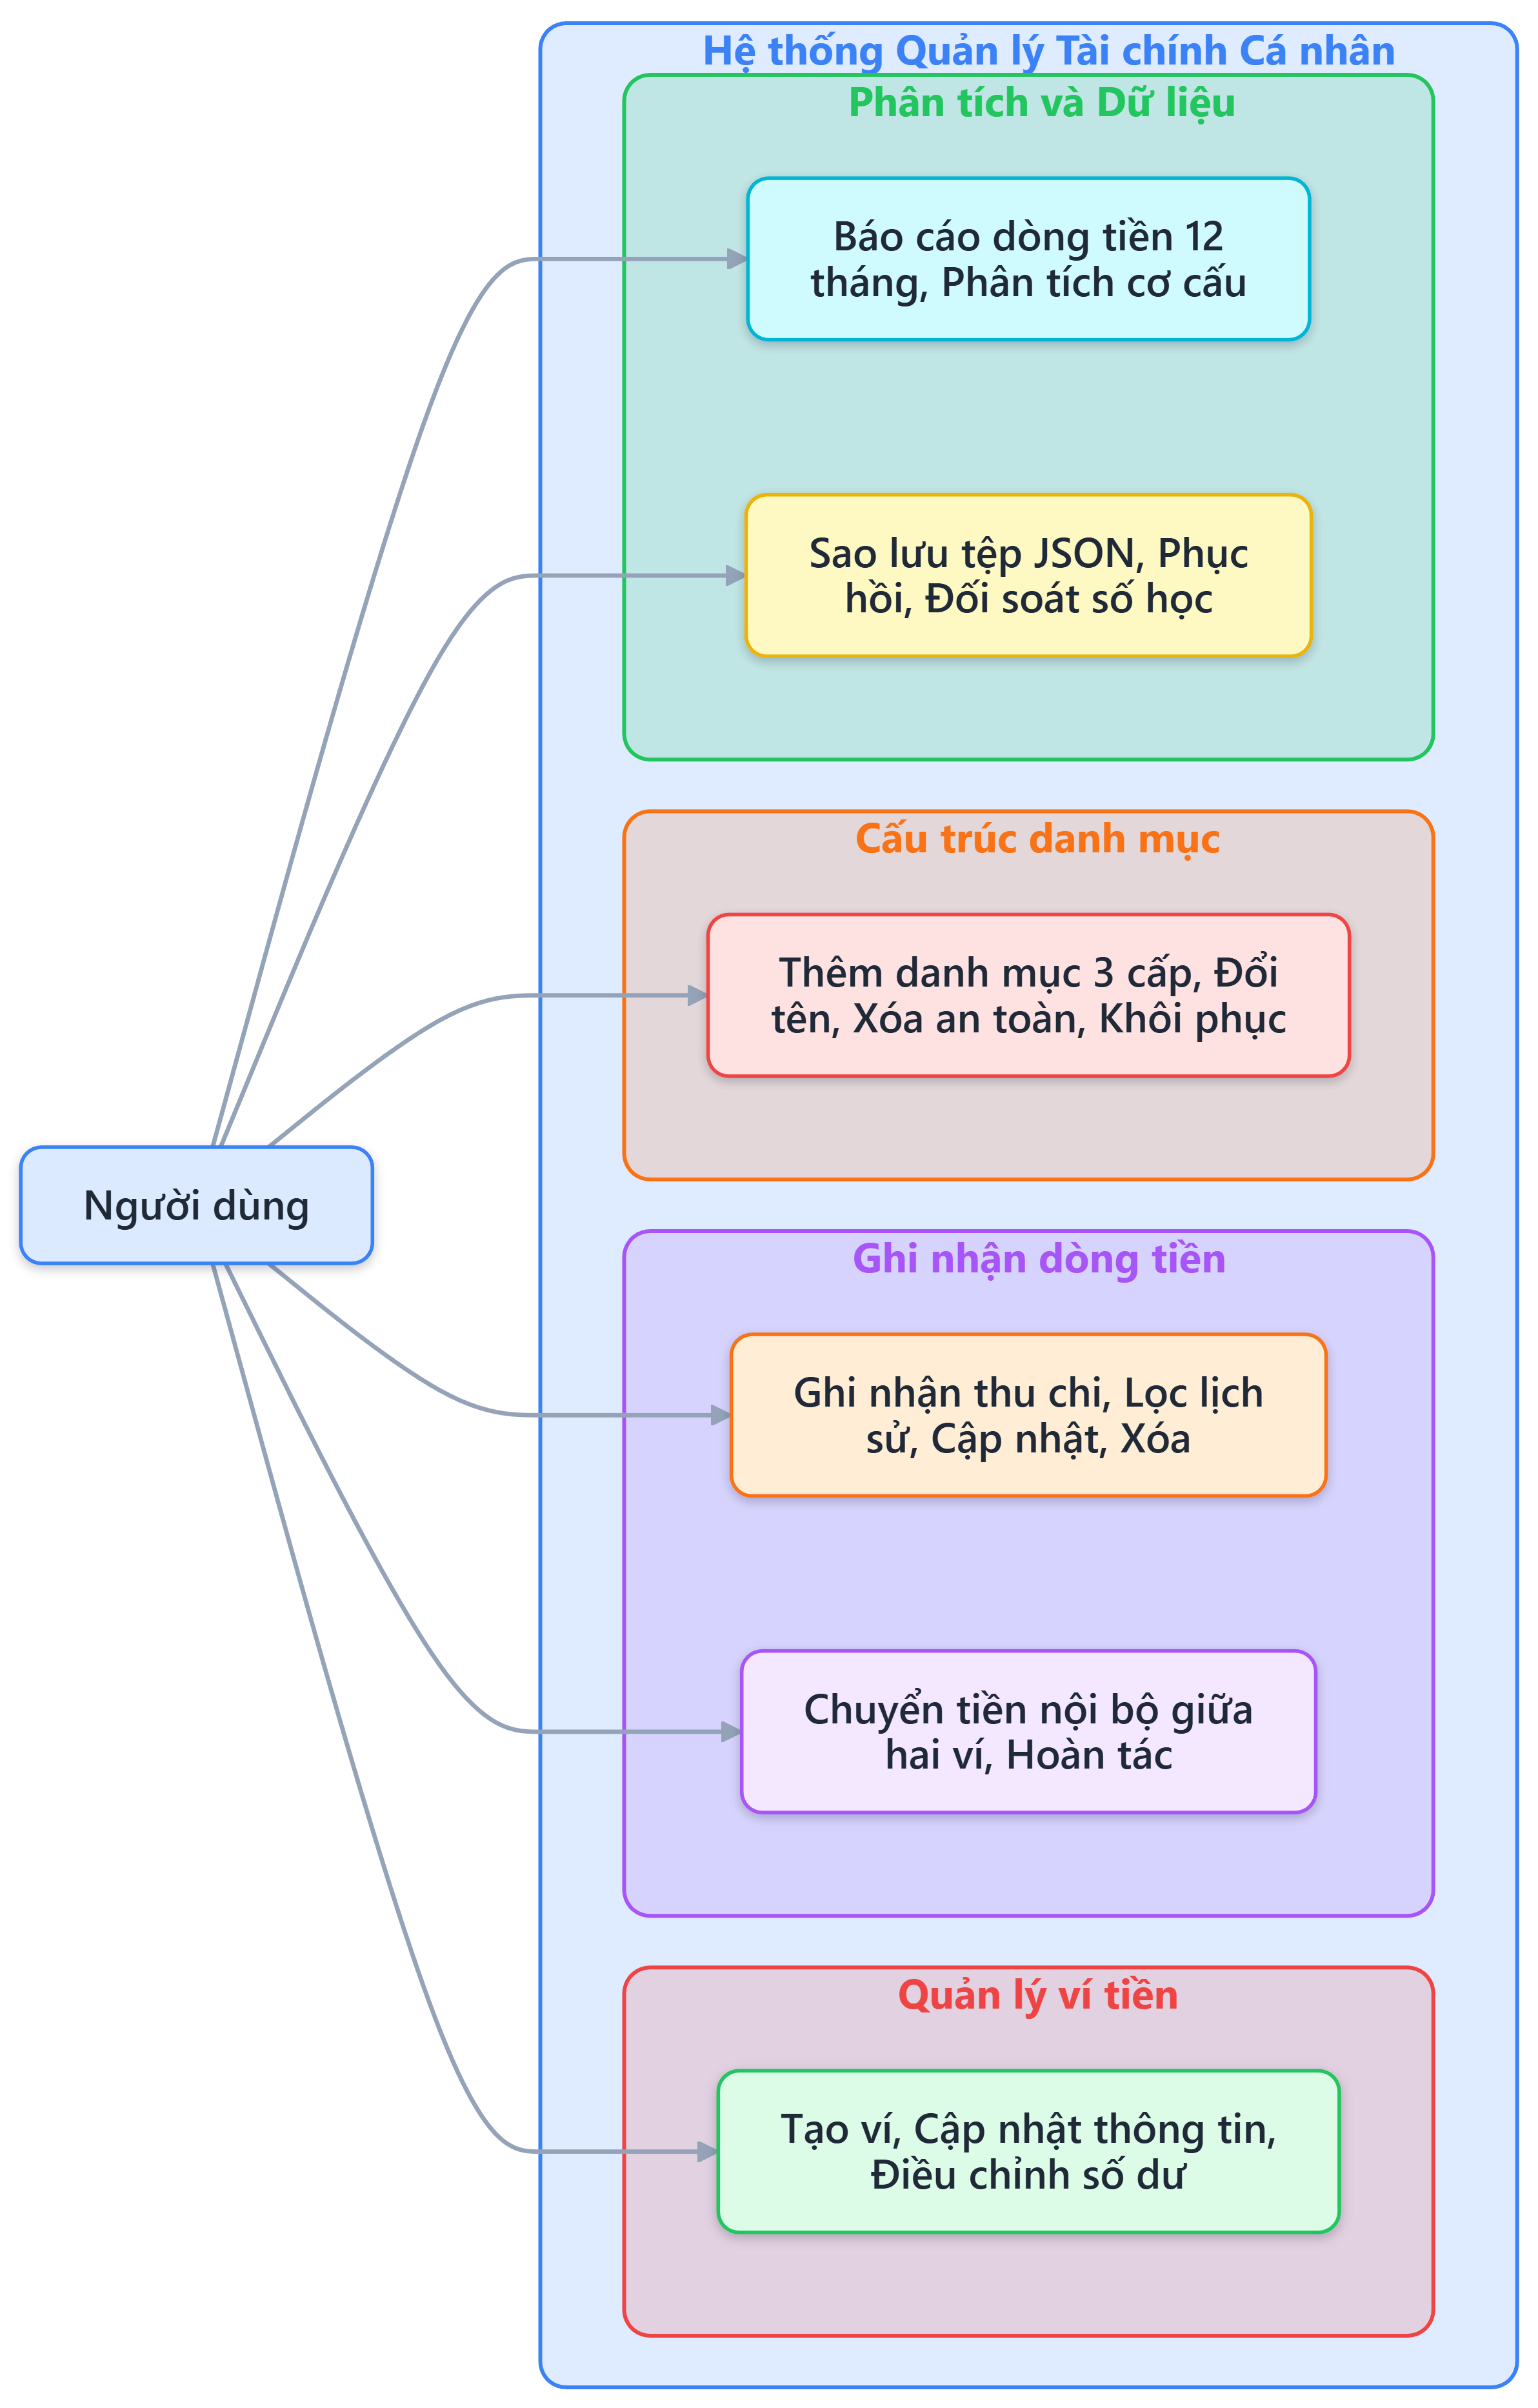
\includegraphics[width=0.85\linewidth,height=\textheight,keepaspectratio,alt={Sơ
đồ ca sử dụng tổng quan hệ thống
PFMS}]{imgs/bao-cao-tong-ket-1.png}
\caption{Sơ đồ ca sử dụng tổng quan hệ thống PFMS}
\end{figure}

\section{Yêu cầu chất lượng và ràng buộc kỹ
thuật}\label{yuxeau-cux1ea7u-chux1ea5t-lux1b0ux1ee3ng-vuxe0-ruxe0ng-buux1ed9c-kux1ef9-thuux1eadt}

Hệ thống thiết lập các tiêu chí định lượng về chất lượng phần mềm: - Độ
chính xác số học: Dung sai tính toán số học bằng 0. Mọi phép toán nhân
chia tỷ lệ đều tuân thủ làm tròn nửa chẵn với 4 chữ số thập phân trước
khi chuyển về định dạng hiển thị. - Hiệu năng phản hồi: Thời gian xử lý
cho các tác vụ thêm mới, cập nhật hoặc tính toán lại số dư không vượt
quá 200 mili-giây với quy mô dữ liệu cá nhân lên đến 50.000 bản ghi. -
Tính tin cậy và lưu trữ tệp: Quá trình lưu trữ tệp JSON áp dụng cơ chế
ghi tệp nguyên tử qua tệp tạm trung gian, ngăn chặn hiện tượng hỏng tệp
khi ứng dụng bị tắt đột ngột. - Khả năng bảo trì: Mã nguồn tuân thủ
triệt để tính đóng gói, phân tách giao diện và trừu tượng hóa, cho phép
thay thế cơ chế lưu trữ mà không ảnh hưởng đến tầng nghiệp vụ. - Môi
trường vận hành: Ứng dụng chạy trên nền tảng Java 17 LTS, tương thích
hoàn toàn trên các hệ điều hành Windows, macOS và Linux.

\chapter{Phân tích hướng đối
tượng}\label{phuxe2n-tuxedch-hux1b0ux1edbng-ux111ux1ed1i-tux1b0ux1ee3ng}

\section{Mô hình khái niệm và các đối tượng nghiệp
vụ}\label{muxf4-huxecnh-khuxe1i-niux1ec7m-vuxe0-cuxe1c-ux111ux1ed1i-tux1b0ux1ee3ng-nghiux1ec7p-vux1ee5}

Trong giai đoạn phân tích hướng đối tượng, hệ thống phân tách rõ ràng
giữa hai nhóm khái niệm căn bản của miền tài chính: Thực thể mang bản
sắc định danh độc lập và Đối tượng giá trị đại diện cho các đại lượng đo
lường bất biến.

Danh mục các lớp thực thể:
\begin{enumerate}
\def\labelenumi{\arabic{enumi}.}
\tightlist
\item
  \passthrough{\lstinline!Wallet!}: Đại diện cho ví tài chính cá nhân. Mỗi
  ví có mã định danh duy nhất (UUID), tên ví, ghi chú, trạng thái ví mặc
  định, thời điểm tạo và trạng thái vòng đời.
\item
  \passthrough{\lstinline!IncomeExpenseTransaction!}: Đại diện cho giao dịch
  thu nhập hoặc chi tiêu diễn ra tại một ví xác định, được gán với một
  danh mục phân loại chi tiết.
\item
  \passthrough{\lstinline!TransferTransaction!}: Đại diện cho giao dịch điều
  chuyển tiền giữa hai ví nội bộ, ghi nhận ví nguồn, ví đích và chi phí
  chuyển tiền đi kèm nếu có.
\item
  \passthrough{\lstinline!TransactionFee!}: Đại diện cho khoản phí phát
  sinh khi thực hiện chuyển tiền. Lớp này có quan hệ hợp thành sinh tử với
  giao dịch chuyển tiền gốc.
\item
  \passthrough{\lstinline!Category!}: Đại diện cho danh mục phân loại chi
  tiết cấp 3 (ví dụ: Ăn uống, Tiền thuê nhà, Tiền lương).
\item
  \passthrough{\lstinline!NeedGroup!}: Đại diện cho nhóm nhu cầu tài chính
  cấp 2 (Nhu cầu thiết yếu, Nhu cầu linh hoạt, Tích lũy đầu tư), đóng vai
  trò phân tầng chi tiêu.
\item
  \passthrough{\lstinline!BalanceAdjustmentRecord!}: Đại diện cho bản ghi
  kiểm kê thực tế khi phát sinh chênh lệch số dư giữa sổ sách và tiền mặt
  thực tế.
\end{enumerate}

Danh mục các đối tượng giá trị:
\begin{enumerate}
\def\labelenumi{\arabic{enumi}.}
\tightlist
\item
  \passthrough{\lstinline!Money!}: Bọc đại lượng tiền tệ với độ chính xác
  cao bằng \passthrough{\lstinline!BigDecimal!} và mã tiền tệ chuẩn hóa
  (mặc định VND). Lớp này hoàn toàn bất biến và cung cấp các phép toán cộng,
  trừ, nhân tỷ lệ an toàn.
\item
  \passthrough{\lstinline!TransactionDate!}: Đóng gói thời điểm diễn ra
  biến động tài chính, đảm bảo ngày giao dịch hợp lệ theo định dạng chuẩn
  ISO-8601 và không vượt quá thời gian thực tế.
\item
  \passthrough{\lstinline!TransactionType!}: Kiểu liệt kê phân định rõ bản
  chất biến động tài chính: \passthrough{\lstinline!INCOME!} (Thu nhập),
  \passthrough{\lstinline!EXPENSE!} (Chi phí),
  \passthrough{\lstinline!TRANSFER!} (Chuyển tiền),
  \passthrough{\lstinline!ADJUSTMENT!} (Điều chỉnh số dư).
\item
  \passthrough{\lstinline!NetCashFlow!}: Giá trị đại số thể hiện dòng tiền
  thuần trong kỳ, tính bằng tổng thu nhập trừ tổng chi phí.
\item
  \passthrough{\lstinline!SavingsRate!}: Tỷ lệ phần trăm tiết kiệm được trên
  tổng thu nhập, phản ánh hiệu quả tích lũy tài chính.
\item
  \passthrough{\lstinline!SpendingStructureShare!}: Tỷ trọng chi tiêu của
  một nhóm hoặc danh mục cụ thể trên tổng chi tiêu toàn hệ thống.
\end{enumerate}

Sơ đồ mô hình miền khái niệm dưới đây thể hiện mối quan hệ ngữ nghĩa
giữa các thực thể và đối tượng giá trị:

\begin{figure}
\centering
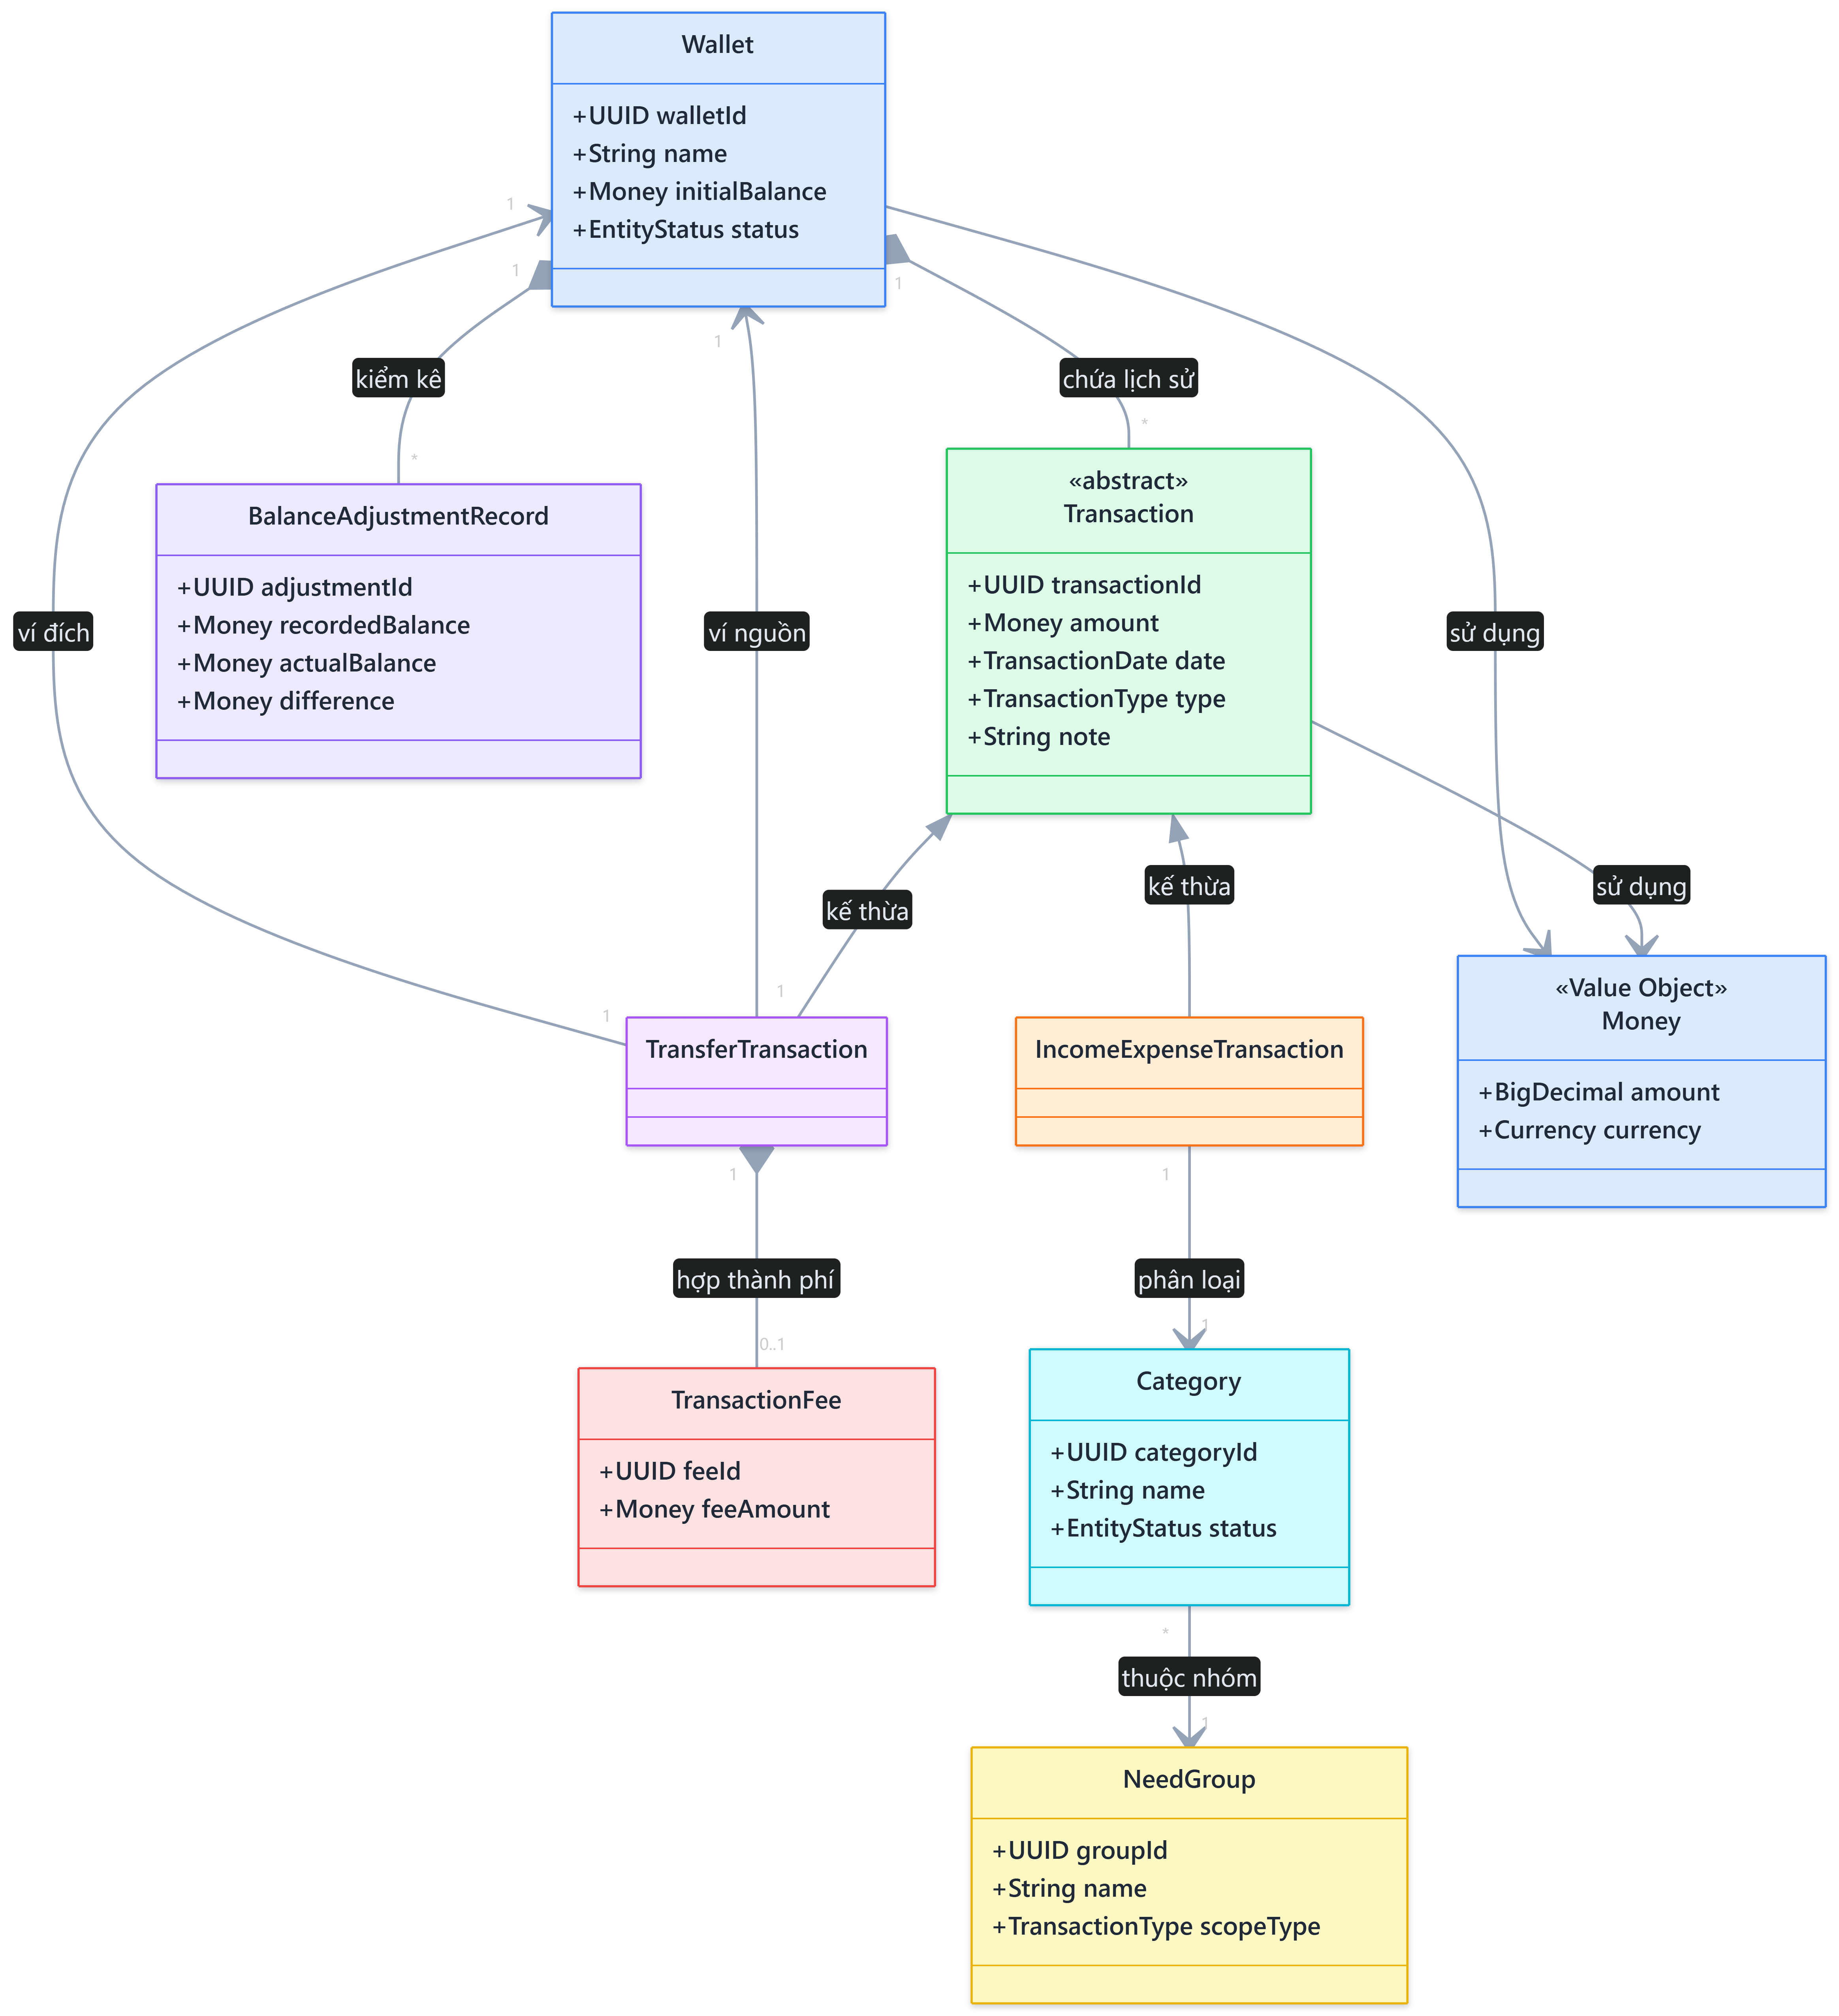
\includegraphics[width=0.85\linewidth,height=\textheight,keepaspectratio,alt={Mô
hình khái niệm và các thực thể nghiệp vụ cốt
lõi}]{imgs/bao-cao-tong-ket-2.png}
\caption{Mô hình khái niệm và các thực thể nghiệp vụ cốt lõi}
\end{figure}

\section{Sơ đồ tương tác tuần tự cấp hệ
thống}\label{sux1a1-ux111ux1ed3-tux1b0ux1a1ng-tuxe1c-tuux1ea7n-tux1ef1-cux1ea5p-hux1ec7-thux1ed1ng}

Sơ đồ tuần tự hệ thống mô tả cách người dùng gửi các thông điệp nghiệp
vụ đến ranh giới hệ thống dạng hộp đen và nhận lại kết quả phản hồi.

Sơ đồ dưới đây minh họa luồng thực hiện thao tác chuyển tiền nội bộ giữa
hai ví:

\begin{figure}
\centering
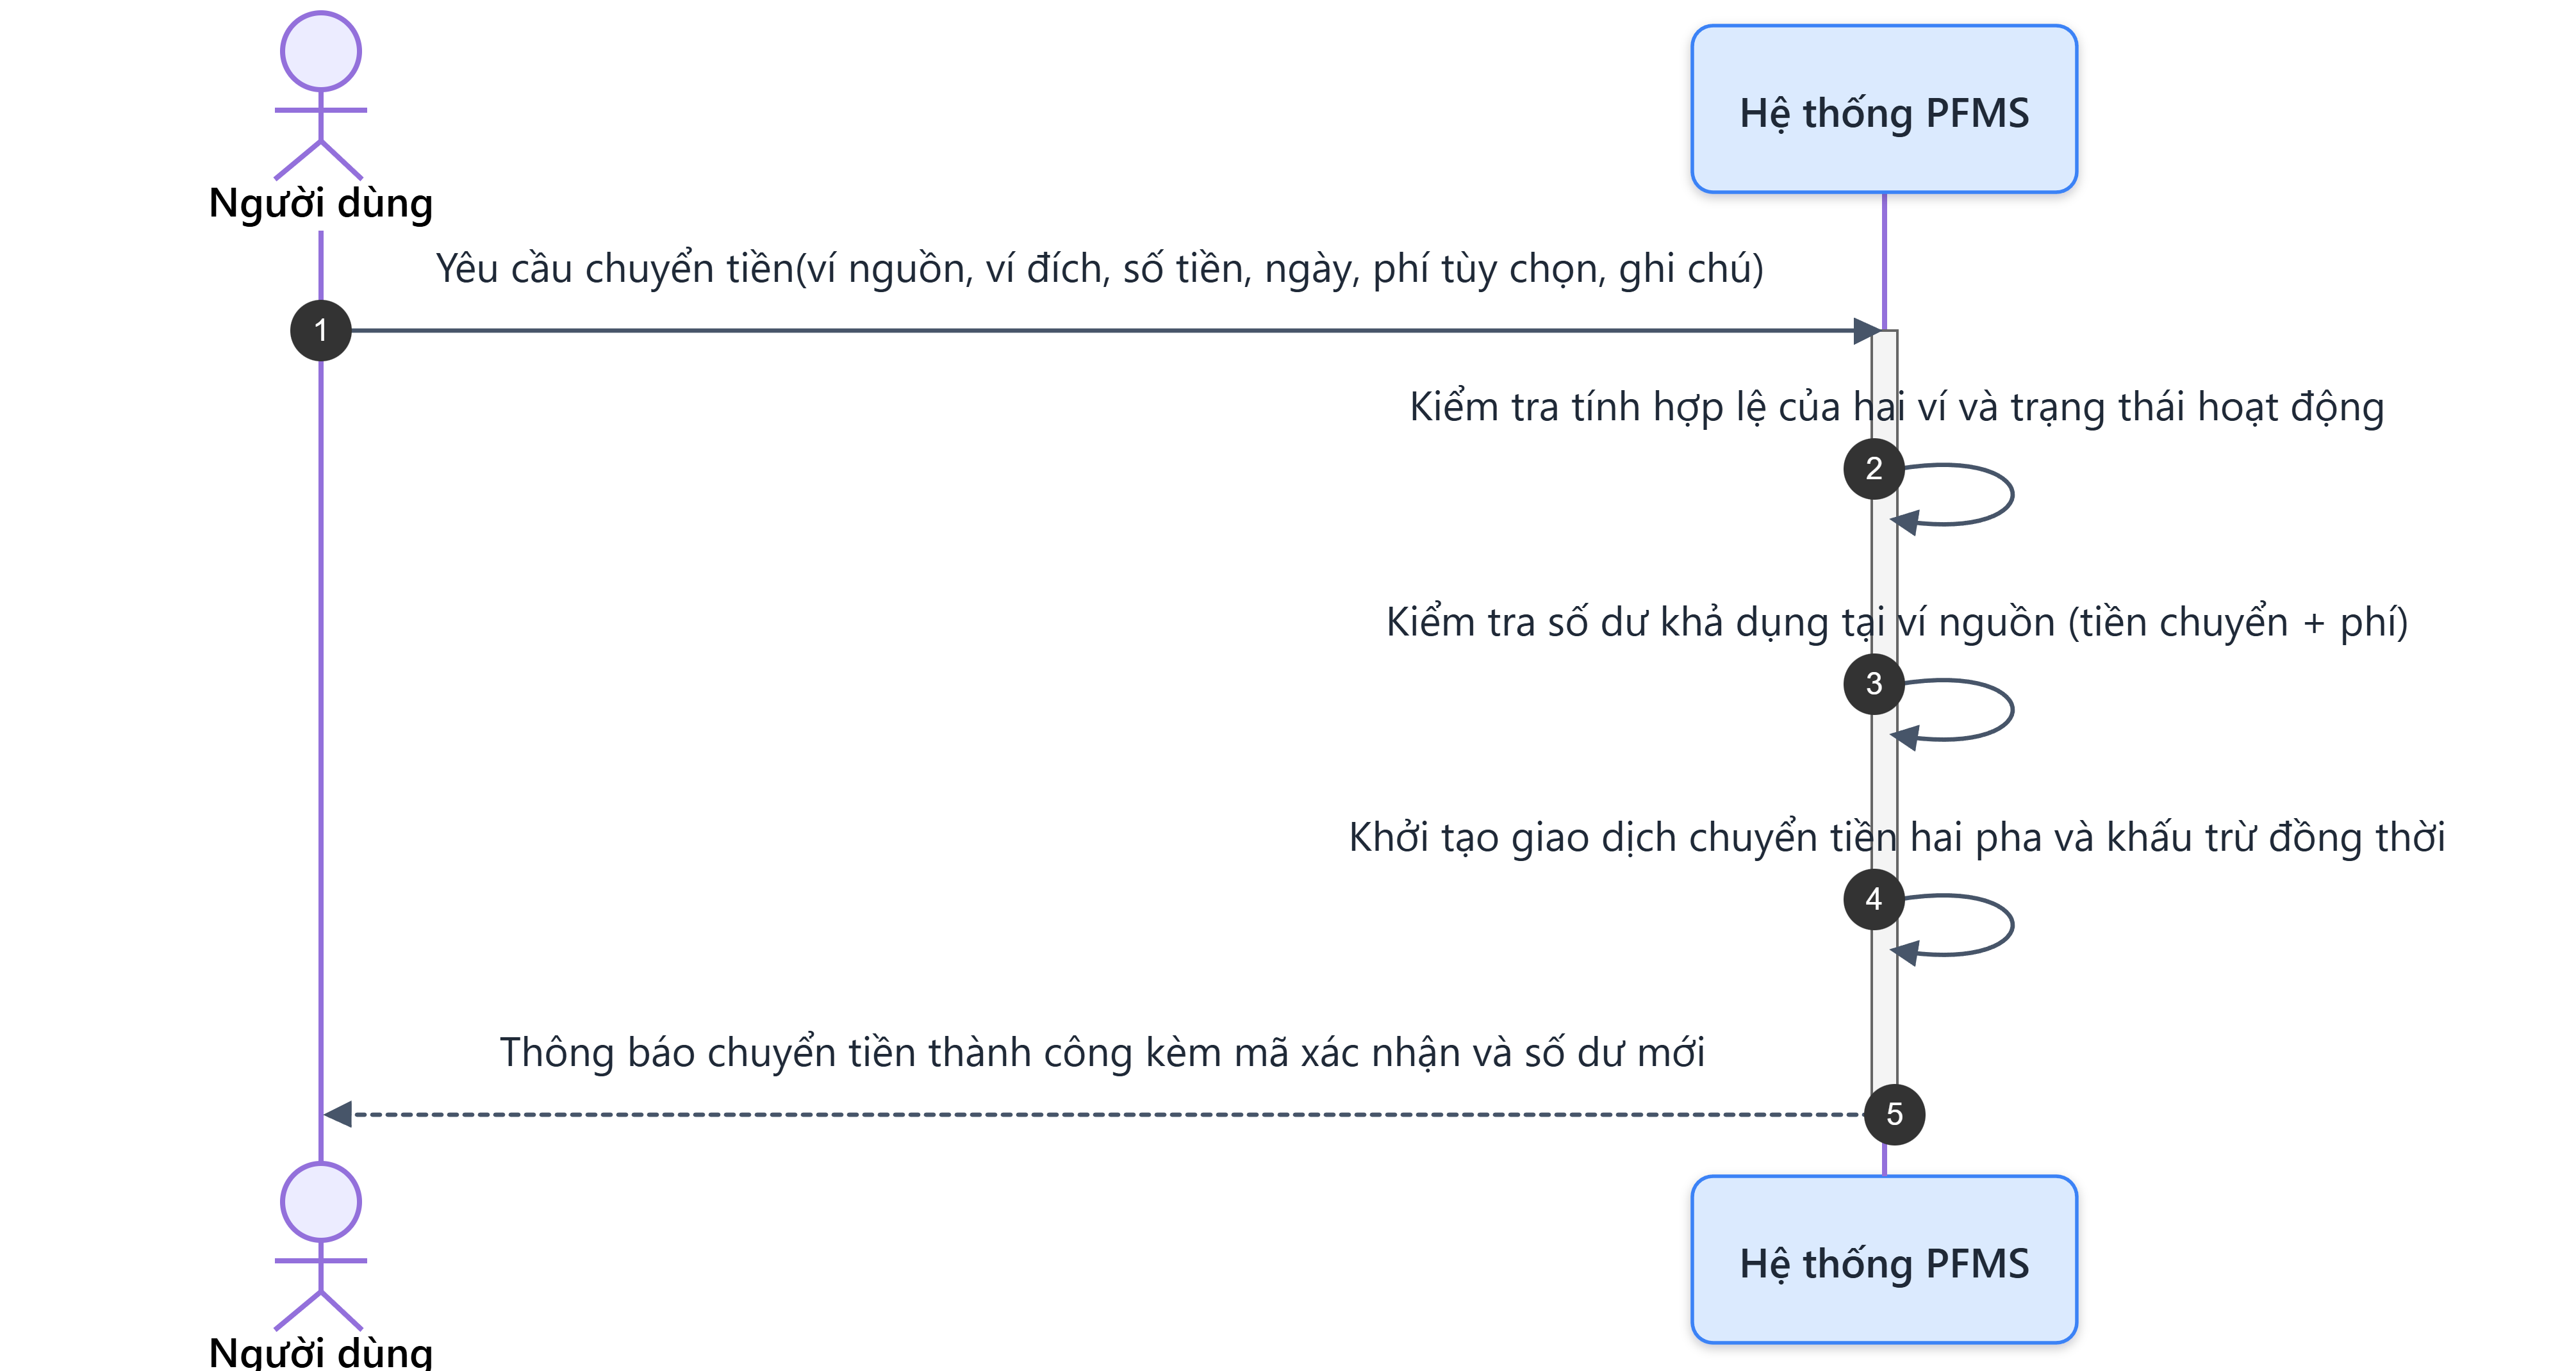
\includegraphics[width=0.85\linewidth,height=\textheight,keepaspectratio,alt={Sơ
đồ tương tác tuần tự cấp hệ thống cho nghiệp vụ chuyển tiền nội bộ giữa
hai ví}]{imgs/bao-cao-tong-ket-3.png}
\caption{Sơ đồ tương tác tuần tự cấp hệ thống cho nghiệp vụ chuyển tiền
nội bộ giữa hai ví}
\end{figure}

\section{Ràng buộc thực hiện thao tác nghiệp
vụ}\label{ruxe0ng-buux1ed9c-thux1ef1c-hiux1ec7n-thao-tuxe1c-nghiux1ec7p-vux1ee5}

Mọi biến động dữ liệu trong hệ thống đều được kiểm soát bằng các hợp
đồng thao tác định rõ điều kiện tiền đề (Pre-conditions) và kết quả bảo
đảm sau thực thi (Post-conditions).

Hai hợp đồng thao tác đại diện cho các ca sử dụng then chốt:

\begin{enumerate}
\def\labelenumi{\arabic{enumi}.}
\tightlist
\item
  Hợp đồng thao tác ghi nhận thu chi
  (\passthrough{\lstinline!recordIncomeExpense!}):
\end{enumerate}

\begin{itemize}
\tightlist
\item
  Điều kiện tiền đề: Ví tài chính được chọn phải tồn tại và đang ở trạng
  thái hoạt động (\passthrough{\lstinline!ACTIVE!}). Danh mục phân loại
  phải tồn tại, đang hoạt động và có loại biến động trùng khớp với loại
  giao dịch. Số tiền giao dịch phải là một số dương lớn hơn 0.
\item
  Kết quả sau thực thi: Một thể hiện mới của
  \passthrough{\lstinline!IncomeExpenseTransaction!} được tạo lập và lưu
  trữ bền vững. Số dư tính toán của ví được cập nhật tương ứng (tăng lên
  nếu là khoản thu, giảm đi nếu là khoản chi). Sự kiện biến động dòng
  tiền được ghi nhận phục vụ báo cáo.
\end{itemize}

\begin{enumerate}
\def\labelenumi{\arabic{enumi}.}
\setcounter{enumi}{1}
\tightlist
\item
  Hợp đồng thao tác chuyển tiền nội bộ
  (\passthrough{\lstinline!transferFunds!}):
\end{enumerate}

\begin{itemize}
\tightlist
\item
  Điều kiện tiền đề: Ví nguồn và ví đích phải cùng tồn tại trong hệ
  thống, đang hoạt động và có mã định danh khác nhau. Số tiền chuyển và
  số tiền phí (nếu có) phải lớn hơn hoặc bằng 0. Số dư hiện tại của ví
  nguồn phải đủ để chi trả tổng số tiền chuyển và phí phát sinh.
\item
  Kết quả sau thực thi: Một thể hiện
  \passthrough{\lstinline!TransferTransaction!} được tạo lập đồng thời
  với một thể hiện \passthrough{\lstinline!TransactionFee!} nếu có phí.
  Số dư ví nguồn giảm đi đúng bằng tổng số tiền chuyển và phí. Số dư ví
  đích tăng lên đúng bằng số tiền chuyển.
\end{itemize}

\section{Vòng đời và trạng thái của các thực
thể}\label{vuxf2ng-ux111ux1eddi-vuxe0-trux1ea1ng-thuxe1i-cux1ee7a-cuxe1c-thux1ef1c-thux1ec3}

Hệ thống quản lý trạng thái của các thực thể thông qua các tập giá trị
chuẩn mực nhằm bảo vệ tính toàn vẹn lịch sử:

{\def\LTcaptype{none} % do not increment counter
\begin{longtable}[]{@{}
  >{\raggedright\arraybackslash}p{(\linewidth - 4\tabcolsep) * \real{0.3333}}
  >{\raggedright\arraybackslash}p{(\linewidth - 4\tabcolsep) * \real{0.3333}}
  >{\raggedright\arraybackslash}p{(\linewidth - 4\tabcolsep) * \real{0.3333}}@{}}
\toprule\noalign{}
\begin{minipage}[b]{\linewidth}\raggedright
Thực thể
\end{minipage} & \begin{minipage}[b]{\linewidth}\raggedright
Các trạng thái hợp lệ
\end{minipage} & \begin{minipage}[b]{\linewidth}\raggedright
Quy tắc chuyển đổi và bảo toàn dữ liệu
\end{minipage} \\
\midrule\noalign{}
\endhead
\bottomrule\noalign{}
\endlastfoot
\textbf{Ví tiền} & Đang hoạt động (\passthrough{\lstinline!ACTIVE!}),
Lưu trữ (\passthrough{\lstinline!ARCHIVED!}), Đã xóa
(\passthrough{\lstinline!DELETED!}). & Ví mới tạo luôn ở trạng thái hoạt
động. Người dùng có thể chuyển sang trạng thái lưu trữ khi không còn sử
dụng thường xuyên. Thao tác xóa ví áp dụng cơ chế xóa mềm; ví chỉ được
xóa khi toàn bộ giao dịch liên quan đã được xử lý hoặc xác nhận hủy. \\
\textbf{Danh mục} & Đang hoạt động (\passthrough{\lstinline!ACTIVE!}),
Đã xóa (\passthrough{\lstinline!DELETED!}). & Danh mục chỉ được xóa mềm
khi không còn bất kỳ giao dịch nào đang tham chiếu tới. Nếu người dùng
muốn sử dụng lại một danh mục đã xóa, hệ thống hỗ trợ khôi phục về trạng
thái hoạt động mà không làm mất lịch sử cũ. \\
\textbf{Giao dịch} & Đã ghi nhận (\passthrough{\lstinline!RECORDED!}),
Đã hủy (\passthrough{\lstinline!VOIDED!}). & Giao dịch tài chính là bản
ghi bất biến sau khi hoàn tất. Khi người dùng thực hiện xóa giao dịch,
hệ thống không xóa vật lý ngay lập tức mà chuyển trạng thái sang đã hủy,
đồng thời kích hoạt quy trình hoàn tác số dư đối soát an toàn. \\
\end{longtable}
}

\section{Phân định trách nhiệm giữa các thành
phần}\label{phuxe2n-ux111ux1ecbnh-truxe1ch-nhiux1ec7m-giux1eefa-cuxe1c-thuxe0nh-phux1ea7n}

Hệ thống sử dụng kỹ thuật phân tích Robustness theo mô hình Ranh giới,
Điều khiển và Thực thể kết hợp thẻ CRC để phân định rõ vai trò của từng
cấu phần:

\begin{itemize}
\tightlist
\item
  Lớp ranh giới: Đón nhận tương tác từ người dùng, thực hiện kiểm tra sơ
  bộ định dạng dữ liệu đầu vào và hiển thị thông điệp phản hồi (ví dụ:
  \passthrough{\lstinline!TransactionFormBoundary!},
  \passthrough{\lstinline!WalletOverviewBoundary!}).
\item
  Lớp điều khiển: Chứa logic phối hợp luồng nghiệp vụ, kiểm tra các ràng
  buộc tài chính và điều phối các thực thể miền (ví dụ:
  \passthrough{\lstinline!TransactionCoordinator!},
  \passthrough{\lstinline!TransferManager!}).
\item
  Lớp thực thể: Chứa đựng dữ liệu nghiệp vụ và các phương thức nghiệp vụ
  nội tại độc lập với giao diện (ví dụ:
  \passthrough{\lstinline!Wallet!},
  \passthrough{\lstinline!Transaction!},
  \passthrough{\lstinline!Category!}).
\end{itemize}

Bảng phân bổ trách nhiệm theo thẻ CRC cho các thành phần cốt lõi:

{\def\LTcaptype{none} % do not increment counter
\begin{longtable}[]{@{}
  >{\raggedright\arraybackslash}p{(\linewidth - 4\tabcolsep) * \real{0.3333}}
  >{\raggedright\arraybackslash}p{(\linewidth - 4\tabcolsep) * \real{0.3333}}
  >{\raggedright\arraybackslash}p{(\linewidth - 4\tabcolsep) * \real{0.3333}}@{}}
\toprule\noalign{}
\begin{minipage}[b]{\linewidth}\raggedright
Lớp thành phần
\end{minipage} & \begin{minipage}[b]{\linewidth}\raggedright
Trách nhiệm chính
\end{minipage} & \begin{minipage}[b]{\linewidth}\raggedright
Thành phần cộng tác
\end{minipage} \\
\midrule\noalign{}
\endhead
\bottomrule\noalign{}
\endlastfoot
\passthrough{\lstinline!Wallet!} & Quản lý số dư khả dụng, thẩm định khả
năng chi trả, duy trì trạng thái hoạt động và cung cấp thông tin định
danh. & \passthrough{\lstinline!Money!},
\passthrough{\lstinline!Transaction!} \\
\passthrough{\lstinline!IncomeExpenseTransaction!} & Cung cấp thông tin
số tiền, ngày phát sinh, liên kết ví và danh mục phân loại. &
\passthrough{\lstinline!Wallet!}, \passthrough{\lstinline!Category!},
\passthrough{\lstinline!Money!} \\
\passthrough{\lstinline!TransferTransaction!} & Gắn kết hai ví nội bộ,
quản lý chi phí phát sinh và đảm bảo tính cân đối hai đầu chuyển. &
\passthrough{\lstinline!Wallet!},
\passthrough{\lstinline!TransactionFee!},
\passthrough{\lstinline!Money!} \\
\passthrough{\lstinline!Category!} & Định danh phân loại chi tiêu, kiểm
soát tính hợp lệ theo nhóm nhu cầu. &
\passthrough{\lstinline!NeedGroup!} \\
\passthrough{\lstinline!TransactionService!} & Điều phối tiếp nhận yêu
cầu, gọi kiểm tra nghiệp vụ, lưu trữ giao dịch và thông báo biến động. &
\passthrough{\lstinline!TransactionRepository!},
\passthrough{\lstinline!WalletRepository!},
\passthrough{\lstinline!TransactionFactory!} \\
\end{longtable}
}

\chapter{Thiết kế kiến trúc và mô hình
lớp}\label{thiux1ebft-kux1ebf-kiux1ebfn-truxfac-vuxe0-muxf4-huxecnh-lux1edbp}

\section{Mô hình kiến trúc phân
tầng}\label{muxf4-huxecnh-kiux1ebfn-truxfac-phuxe2n-tux1ea7ng}

Hệ thống Quản lý Tài chính Cá nhân áp dụng mô hình kiến trúc phân tầng
hướng tâm gồm 4 tầng phân định rõ ranh giới trách nhiệm, bảo đảm nguyên
tắc phụ thuộc một chiều từ ngoài vào trong:

\begin{figure}
\centering
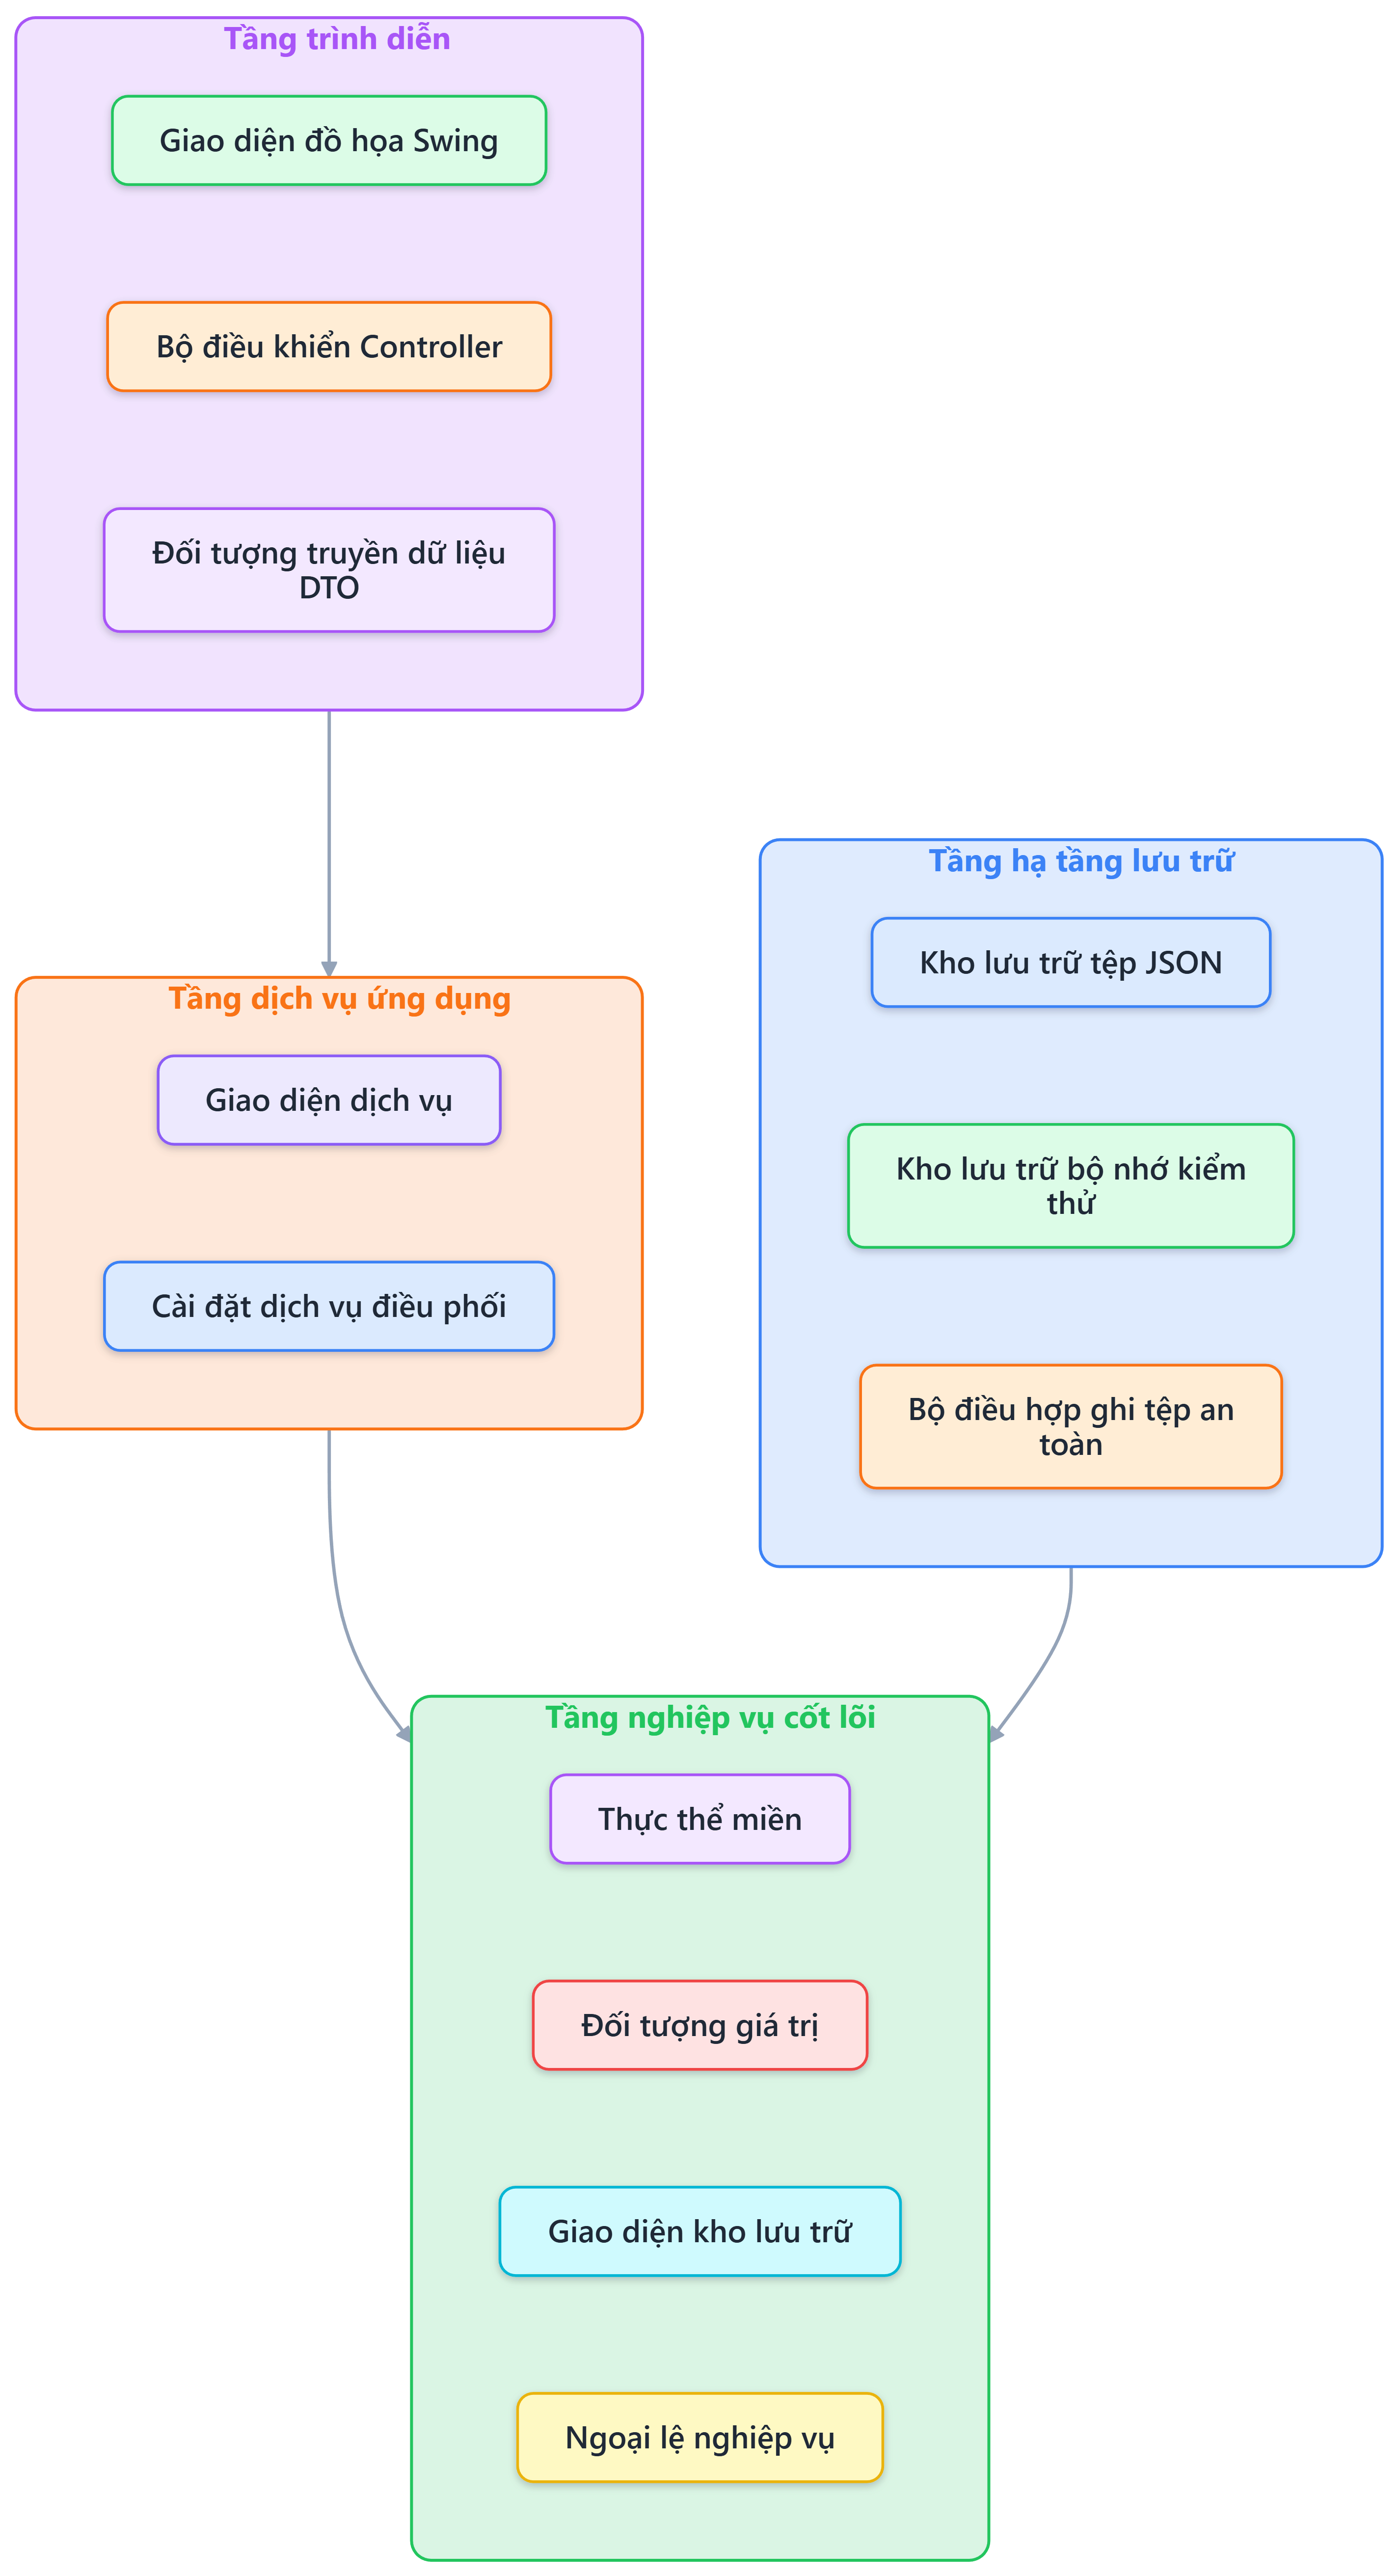
\includegraphics[width=0.85\linewidth,height=\textheight,keepaspectratio,alt={Mô
hình kiến trúc phân tầng 4 lớp của hệ thống
PFMS}]{imgs/bao-cao-tong-ket-4.png}
\caption{Mô hình kiến trúc phân tầng 4 lớp của hệ thống PFMS}
\end{figure}

Trách nhiệm cụ thể của từng tầng: - Tầng Trình diễn
(\passthrough{\lstinline!com.pfms.presentation!}): Chịu trách nhiệm hiển
thị dữ liệu trực quan qua các bảng biểu đồ họa, thu nhận thao tác người
dùng, đóng gói dữ liệu vào các DTO và chuyển tiếp cho tầng dịch vụ xử
lý. Tầng này không chứa logic tính toán tài chính. - Tầng Dịch vụ ứng
dụng (\passthrough{\lstinline!com.pfms.service!}): Đóng vai trò nhạc
trưởng điều phối các ca sử dụng, kiểm tra tính hợp lệ của tham số, quản
lý giao dịch nghiệp vụ và chuyển đổi giữa DTO và thực thể miền. - Tầng
Nghiệp vụ cốt lõi (\passthrough{\lstinline!com.pfms.domain!}): Trái tim
của hệ thống, chứa toàn bộ quy tắc nghiệp vụ tài chính, định nghĩa cấu
trúc dữ liệu thực thể, đối tượng giá trị và giao diện kho lưu trữ. Tầng
này hoàn toàn độc lập, không phụ thuộc vào bất kỳ thư viện giao diện hay
công nghệ lưu trữ cụ thể nào. - Tầng Hạ tầng
(\passthrough{\lstinline!com.pfms.infrastructure!}): Cung cấp cài đặt cụ
thể cho các giao diện kho lưu trữ được định nghĩa ở tầng miền, đảm bảo
lưu trữ tệp bền vững hoặc cung cấp bộ lưu trữ tạm thời trong bộ nhớ phục
vụ kiểm thử.

\section{Thiết kế chi tiết các lớp dữ liệu và thực
thể}\label{thiux1ebft-kux1ebf-chi-tiux1ebft-cuxe1c-lux1edbp-dux1eef-liux1ec7u-vuxe0-thux1ef1c-thux1ec3}

Tầng nghiệp vụ cốt lõi (\passthrough{\lstinline!com.pfms.domain.model!}) đại diện cho hạt nhân kiến trúc của hệ thống PFMS, chịu trách nhiệm quản lý toàn bộ thực thể tài chính, bảo toàn các quy tắc bất biến số học và điều phối hành vi biến động dòng tiền độc lập hoàn toàn khỏi công nghệ giao diện và lưu trữ.

\subsection{Sơ đồ lớp thiết kế và bảng đặc tả thành
phần}\label{sux1a1-ux111ux1ed3-lux1edbp-thiux1ebft-kux1ebf-vuxe0-bux1ea3ng-ux111ux1eb7c-tux1ea3-thuxe0nh-phux1ea7n}

Mô hình lớp thiết kế dưới đây mô tả cấu trúc tĩnh hoàn chỉnh của 8 thực thể miền, các đối tượng giá trị bất biến và các kiểu liệt kê, thể hiện chi tiết danh sách thuộc tính, phương thức nghiệp vụ và các loại quan hệ cấu trúc hướng đối tượng cốt lõi:

\begin{figure}
\centering
\includegraphics[width=0.95\linewidth,height=\textheight,keepaspectratio,alt={Sơ
đồ lớp thiết kế chi tiết các lớp dữ liệu và thực thể
miền}]{imgs/bao-cao-tong-ket-5.png}
\caption{Sơ đồ lớp thiết kế chi tiết các lớp dữ liệu và thực thể miền}
\end{figure}

Nhằm hiện thực hóa mô hình miền giàu hành vi và triệt tiêu hoàn toàn hiện tượng suy thoái dữ liệu, cấu trúc tĩnh trên được quy định vai trò nghiệp vụ, thuộc tính và phương thức tác vụ cụ thể cho từng thành phần như sau:

{\def\LTcaptype{none} % do not increment counter
\begingroup
\renewcommand{\arraystretch}{1.25}
\fontsize{9pt}{12pt}\selectfont
\begin{longtable}[]{@{}
  >{\raggedright\arraybackslash}p{(\linewidth - 6\tabcolsep) * \real{0.2000}}
  >{\raggedright\arraybackslash}p{(\linewidth - 6\tabcolsep) * \real{0.2700}}
  >{\raggedright\arraybackslash}p{(\linewidth - 6\tabcolsep) * \real{0.2400}}
  >{\raggedright\arraybackslash}p{(\linewidth - 6\tabcolsep) * \real{0.2900}}@{}}
\toprule\noalign{}
\begin{minipage}[b]{\linewidth}\raggedright
\textbf{Lớp}
\end{minipage} & \begin{minipage}[b]{\linewidth}\raggedright
\textbf{Thuộc tính}
\end{minipage} & \begin{minipage}[b]{\linewidth}\raggedright
\textbf{Phương thức}
\end{minipage} & \begin{minipage}[b]{\linewidth}\raggedright
\textbf{Vai trò nghiệp vụ}
\end{minipage} \\
\midrule\noalign{}
\endhead
\bottomrule\noalign{}
\endlastfoot
\textbf{\texttt{Wallet}} &
\texttt{id: UUID}\newline
\texttt{name: EntityName}\newline
\texttt{currentBalance: Money}\newline
\texttt{state: WalletState}\newline
\texttt{defaultWallet: boolean} &
\texttt{credit(Money)}\newline
\texttt{debit(Money)}\newline
\texttt{adjustBalance(...)}\newline
\texttt{archive()}, \texttt{activate()},\newline
\texttt{delete()} &
Quản lý nguồn tiền khả dụng, trực tiếp thực thi biến động số dư và kiểm soát vòng đời ví. Luôn bảo toàn số dư không âm (\texttt{currentBalance >= 0}). \\
\midrule\noalign{}
\textbf{\texttt{Transaction}} &
\texttt{transactionId: UUID}\newline
\texttt{amount: Money}\newline
\texttt{transactionDate: Date}\newline
\texttt{note: Note}\newline
\texttt{fee: TransactionFee} &
\texttt{applyToWallet()}\newline
\texttt{revertFromWallet()}\newline
\texttt{getAmount()}\newline
\texttt{getFee()} &
Lớp trừu tượng đóng vai trò khuôn mẫu chung, quy định hợp đồng đa hình tác động và hoàn tác số dư cho mọi biến động dòng tiền. \\
\midrule\noalign{}
\textbf{\texttt{IncomeExpense-}}\newline
\textbf{\texttt{Transaction}} &
\texttt{transactionType:}\newline
\texttt{\ \ TransactionType}\newline
\texttt{wallet: Wallet}\newline
\texttt{category: Category} &
\texttt{applyToWallet()}\newline
\texttt{revertFromWallet()}\newline
\texttt{getWallet()}\newline
\texttt{getCategory()} &
Hiện thực hóa giao dịch thu chi gắn với một danh mục phân loại mục đích; tự động hạch toán chi phí phát sinh đi kèm nếu có. \\
\midrule\noalign{}
\textbf{\texttt{Transfer-}}\newline
\textbf{\texttt{Transaction}} &
\texttt{sourceWallet: Wallet}\newline
\texttt{destinationWallet:}\newline
\texttt{\ \ Wallet} &
\texttt{applyToWallet()}\newline
\texttt{revertFromWallet()}\newline
\texttt{getSourceWallet()}\newline
\texttt{getDestination-}\newline
\texttt{\ \ Wallet()} &
Hiện thực hóa chuyển tiền hai chiều giữa ví nguồn và ví đích theo cơ chế nguyên tử bảo toàn tổng tài sản; hỗ trợ phí chuyển tiền. \\
\midrule\noalign{}
\textbf{\texttt{TransactionFee}} &
\texttt{feeId: UUID}\newline
\texttt{parentTransactionId:}\newline
\texttt{\ \ UUID}\newline
\texttt{amount: Money}\newline
\texttt{wallet: Wallet}\newline
\texttt{category: Category} &
\texttt{applyFee()}\newline
\texttt{revertFee()}\newline
\texttt{getAmount()}\newline
\texttt{getFeeId()} &
Đại diện cho khoản chi phí phát sinh gắn liền sinh tử với giao dịch gốc, được khấu trừ trực tiếp tại ví phát lệnh giao dịch. \\
\midrule\noalign{}
\textbf{\texttt{Category}} &
\texttt{categoryId: UUID}\newline
\texttt{name: EntityName}\newline
\texttt{needGroupId: UUID}\newline
\texttt{transactionType:}\newline
\texttt{\ \ TransactionType}\newline
\texttt{status: EntityStatus} &
\texttt{rename(String)}\newline
\texttt{markDeleted()}\newline
\texttt{restore(boolean)}\newline
\texttt{getCategoryId()} &
Danh mục thu chi chi tiết cấp 3 gán nhãn mục đích cho từng giao dịch; áp dụng cơ chế xóa mềm nhằm bảo vệ tính toàn vẹn dữ liệu lịch sử. \\
\midrule\noalign{}
\textbf{\texttt{NeedGroup}} &
\texttt{needGroupId: UUID}\newline
\texttt{name: EntityName}\newline
\texttt{transactionType:}\newline
\texttt{\ \ TransactionType}\newline
\texttt{status: EntityStatus}\newline
\texttt{categories: List} &
\texttt{addCategory(...)}\newline
\texttt{removeCategory(...)}\newline
\texttt{rename(String)} &
Quản lý nhóm nhu cầu tài chính cấp 2 (Thiết yếu, Linh hoạt, Tích lũy) gom cụm các danh mục con phục vụ phân tích cơ cấu chi tiêu. \\
\midrule\noalign{}
\textbf{\texttt{Balance-}}\newline
\textbf{\texttt{Adjustment-}}\newline
\textbf{\texttt{Record}} &
\texttt{recordId: UUID}\newline
\texttt{walletId: UUID}\newline
\texttt{previousBalance: Money}\newline
\texttt{actualBalance: Money}\newline
\texttt{difference: Money} &
\texttt{getPreviousBalance()}\newline
\texttt{getActualBalance()}\newline
\texttt{getDifference()} &
Lưu vết kiểm toán sự kiện đối soát kiểm kê tiền thực tế so với sổ sách; ghi nhận độ lệch đại số để điều chỉnh số dư về đúng thực tế. \\
\midrule\noalign{}
\textbf{\texttt{Money}} &
\texttt{amount: BigDecimal}\newline
\texttt{currency: Currency} &
\texttt{add(Money)}\newline
\texttt{subtract(Money)}\newline
\texttt{multiply(BigDecimal)}\newline
\texttt{isPositive()}, \texttt{isZero()} &
Đối tượng giá trị bất biến bọc đại lượng tiền tệ độ chính xác cao; áp dụng làm tròn nửa chẵn (\texttt{HALF\_EVEN}), loại trừ sai số dấu phẩy động. \\
\midrule\noalign{}
\textbf{\texttt{TransactionDate}} &
\texttt{date: LocalDate} &
\texttt{getDate()}\newline
\texttt{isBefore(...)}\newline
\texttt{isAfter(...)} &
Đối tượng giá trị bất biến bọc mốc ngày phát sinh giao dịch theo ISO-8601; chặn ngày vượt quá thời điểm hiện tại của hệ thống. \\
\midrule\noalign{}
\textbf{\texttt{EntityName}} \&\newline
\textbf{\texttt{Note}} &
\texttt{value: String} &
\texttt{getValue()}\newline
\texttt{Note.empty()} &
Đối tượng giá trị chuẩn hóa chuỗi ký tự tên gọi (1--50 ký tự) và ghi chú diễn giải (tối đa 255 ký tự kèm cơ chế đối tượng rỗng). \\
\end{longtable}
\endgroup
}

\subsection{Phân tích các quan hệ cấu trúc giữa các lớp trong mô hình thiết
kế}\label{phuxe2n-tuxedch-cuxe1c-quan-hux1ec7-cux1ea5u-truxe1c-giux1eefa-cuxe1c-lux1edbp-trong-muxf4-huxecnh-thiux1ebft-kux1ebf}

Mô hình lớp miền nghiệp vụ của hệ thống PFMS hiện thực hóa 4 loại quan hệ cấu trúc chuẩn mực trong UML, định hình luồng tương tác và ràng buộc vòng đời giữa các thực thể:

\begin{enumerate}
\def\labelenumi{\arabic{enumi}.}
\item
  \textbf{Quan hệ kế thừa (Generalization/Inheritance):} Hai thực thể giao dịch cụ thể \passthrough{\lstinline!IncomeExpenseTransaction!} và \passthrough{\lstinline!TransferTransaction!} kế thừa trực tiếp từ lớp cơ sở trừu tượng \passthrough{\lstinline!Transaction!}. Mối quan hệ này cho phép trừu tượng hóa các trường trạng thái và hành vi chung của dòng tiền (\passthrough{\lstinline!transactionId!}, \passthrough{\lstinline!amount!}, \passthrough{\lstinline!transactionDate!}, \passthrough{\lstinline!note!}, \passthrough{\lstinline!fee!}), đồng thời quy định hợp đồng đa hình bắt buộc cho các lớp con.
\item
  \textbf{Quan hệ hợp thành (Composition):} Lớp \passthrough{\lstinline!TransactionFee!} được liên kết với \passthrough{\lstinline!Transaction!} thông qua quan hệ hợp thành với bội số 1 đến 0..1 (mỗi giao dịch có thể phát sinh tối đa một bản ghi chi phí đi kèm). Bản ghi chi phí phụ thuộc hoàn toàn vào vòng đời của giao dịch chủ quản. Khi giao dịch chuyển tiền được tạo lập, bản ghi phí được sinh ra đồng thời; khi giao dịch bị hoàn tác hoặc hủy bỏ, bản ghi phí được xử lý đồng bộ, triệt tiêu nguy cơ phát sinh dữ liệu chi phí mồ côi.
\item
  \textbf{Quan hệ kết tập (Aggregation):} Thực thể \passthrough{\lstinline!NeedGroup!} thiết lập quan hệ kết tập với tập hợp các \passthrough{\lstinline!Category!} cấp dưới thông qua bội số 1 đến * (một nhóm nhu cầu chứa danh sách nhiều danh mục con qua thuộc tính \passthrough{\lstinline!categories!}). Quan hệ này phân tách ranh giới rõ ràng: nhóm nhu cầu đóng vai trò gom cụm logic để tính toán tỷ trọng phân bổ dòng tiền, nhưng các danh mục con vẫn duy trì định danh và vòng đời độc lập, cho phép người dùng đổi tên hoặc xóa mềm từng danh mục mà không làm phá vỡ toàn bộ cấu trúc của nhóm cha.
\item
  \textbf{Quan hệ liên kết và chiều điều hướng (Association \& Navigability):} Giao dịch thu chi \passthrough{\lstinline!IncomeExpenseTransaction!} duy trì liên kết một chiều (* \(\to\) 1) tới \passthrough{\lstinline!Category!} để xác định mục đích chi tiêu và tới \passthrough{\lstinline!Wallet!} để xác định tài khoản phát sinh. Giao dịch chuyển tiền \passthrough{\lstinline!TransferTransaction!} duy trì liên kết tới hai ví độc lập: \passthrough{\lstinline!sourceWallet!} (ví trích tiền kèm phí) và \passthrough{\lstinline!destinationWallet!} (ví nhận tiền). Bản ghi \passthrough{\lstinline!BalanceAdjustmentRecord!} duy trì liên kết một chiều tới \passthrough{\lstinline!Wallet!} được kiểm kê để lưu vết đối soát.
\end{enumerate}

\subsection{Hiện thực hóa bốn tính chất cốt lõi của lập trình hướng đối
tượng}\label{hiux1ec7n-thux1ef1c-huxf3a-bux1ed1n-tuxednh-chux1ea5t-cux1ed1t-luxf5i-cux1ee7a-lux1eadp-truxecnh-hux1b0ux1edbng-ux111ux1ed1i-tux1b0ux1ee3ng}

Kiến trúc tầng miền của PFMS vận dụng sâu sắc 4 nguyên lý nền tảng của lập trình hướng đối tượng nhằm bảo vệ tối đa tính toàn vẹn nghiệp vụ tài chính:

\begin{enumerate}
\def\labelenumi{\arabic{enumi}.}
\item
  \textbf{Tính đóng gói (Encapsulation):} Toàn bộ trường dữ liệu của mọi thực thể đều được khai báo với phạm vi truy cập \passthrough{\lstinline!private!} hoặc \passthrough{\lstinline!protected!}, loại bỏ triệt để các phương thức setter tự do nhằm ngăn chặn việc biến đổi trạng thái tùy tiện từ bên ngoài. Các đại lượng tài chính và mốc thời gian được đóng gói vào các Đối tượng giá trị bất biến (\passthrough{\lstinline!Money!}, \passthrough{\lstinline!TransactionDate!}, \passthrough{\lstinline!EntityName!}, \passthrough{\lstinline!Note!}). Các phép toán số học trên \passthrough{\lstinline!Money!} luôn sinh ra một đối tượng mới hoàn toàn độc lập, áp dụng quy tắc làm tròn nửa chẵn (\passthrough{\lstinline!HALF_EVEN!}) với thang đo 4 chữ số thập phân, triệt tiêu hoàn toàn sai số dấu phẩy động và các tác dụng phụ ngoài ý muốn.
\item
  \textbf{Tính trừu tượng (Abstraction):} Lớp cơ sở trừu tượng \passthrough{\lstinline!Transaction!} chỉ quy định giao ước ``CÁI GÌ'' cần thực hiện thông qua chữ ký của hai phương thức trừu tượng \passthrough{\lstinline!applyToWallet()!} và \passthrough{\lstinline!revertFromWallet()!}, che giấu hoàn toàn chi tiết ``LÀM NHƯ THẾ NÀO''. Tính trừu tượng còn thể hiện ở mô hình máy trạng thái \passthrough{\lstinline!WalletState!}: các hành vi nạp tiền, chi tiền, chuyển đổi trạng thái của \passthrough{\lstinline!Wallet!} được trừu tượng hóa qua giao diện trạng thái, giải phóng thực thể ví khỏi các khối lệnh rẽ nhánh phức tạp.
\item
  \textbf{Tính kế thừa (Inheritance):} Triệt tiêu hoàn toàn sự trùng lặp mã nguồn (nguyên lý DRY): các lớp con \passthrough{\lstinline!IncomeExpenseTransaction!} và \passthrough{\lstinline!TransferTransaction!} tái sử dụng toàn bộ định danh, mốc thời gian, số tiền và các phương thức kiểm tra điều kiện biên từ lớp cha \passthrough{\lstinline!Transaction!}. Lớp con chỉ tập trung mở rộng các thuộc tính nghiệp vụ đặc thù: \passthrough{\lstinline!IncomeExpenseTransaction!} mở rộng thêm liên kết danh mục phân loại mục đích; \passthrough{\lstinline!TransferTransaction!} mở rộng thêm liên kết ví đích hai chiều.
\item
  \textbf{Tính đa hình (Polymorphism):} Hiện thực hóa cơ chế liên kết động: Cùng một lời gọi phương thức \passthrough{\lstinline!transaction.applyToWallet()!}, hệ thống tự động định tuyến hành vi tại thời điểm thực thi. Nếu là giao dịch thu chi, hệ thống tác động lên một ví duy nhất; nếu là chuyển tiền, hệ thống trích nợ ví nguồn và ghi có vào ví đích theo cơ chế nguyên tử. Nhờ tính đa hình, tầng dịch vụ (\passthrough{\lstinline!TransactionServiceImpl!}) và các thuật toán tổng hợp báo cáo chỉ cần tương tác qua kiểu tham chiếu cha \passthrough{\lstinline!Transaction!}. Khi hệ thống cần bổ sung loại giao dịch mới trong tương lai, mã nguồn điều phối hoàn toàn không phải thay đổi, thỏa mãn xuất sắc nguyên lý Đóng/Mở.
\end{enumerate}

\section{Thiết kế các dịch vụ xử lý nghiệp
vụ}\label{thiux1ebft-kux1ebf-cuxe1c-dux1ecbch-vux1ee5-xux1eed-luxfd-nghiux1ec7p-vux1ee5}

Tầng dịch vụ ứng dụng được phân rã thành 6 giao diện chuyên biệt, đảm
bảo tính gắn kết cao và tuân thủ nguyên lý phân tách giao diện:

{\def\LTcaptype{none} % do not increment counter
\begin{longtable}[]{@{}
  >{\raggedright\arraybackslash}p{(\linewidth - 4\tabcolsep) * \real{0.3333}}
  >{\raggedright\arraybackslash}p{(\linewidth - 4\tabcolsep) * \real{0.3333}}
  >{\raggedright\arraybackslash}p{(\linewidth - 4\tabcolsep) * \real{0.3333}}@{}}
\toprule\noalign{}
\begin{minipage}[b]{\linewidth}\raggedright
Giao diện dịch vụ
\end{minipage} & \begin{minipage}[b]{\linewidth}\raggedright
Lớp cài đặt chính
\end{minipage} & \begin{minipage}[b]{\linewidth}\raggedright
Chức năng điều phối trọng tâm
\end{minipage} \\
\midrule\noalign{}
\endhead
\bottomrule\noalign{}
\endlastfoot
\passthrough{\lstinline!WalletService!} &
\passthrough{\lstinline!WalletServiceImpl!} & Quản lý vòng đời ví, điều
phối kiểm kê điều chỉnh số dư, tổng hợp số dư thực tế tính toán từ toàn
bộ dòng tiền lịch sử. \\
\passthrough{\lstinline!TransactionService!} &
\passthrough{\lstinline!TransactionServiceImpl!} & Xử lý ghi nhận thu
chi, thực hiện tìm kiếm và lọc giao dịch đa tiêu chí, điều phối cập nhật
và xóa giao dịch an toàn. \\
\passthrough{\lstinline!TransferService!} &
\passthrough{\lstinline!TransferServiceImpl!} & Điều phối chuyển tiền
nguyên tử hai pha giữa hai ví, tính toán chi phí, xử lý hoàn tác giao
dịch chuyển tiền. \\
\passthrough{\lstinline!CategoryService!} &
\passthrough{\lstinline!CategoryServiceImpl!} & Quản trị cây danh mục 3
cấp, kiểm tra ràng buộc toàn vẹn trước khi cho phép xóa mềm hoặc khôi
phục danh mục. \\
\passthrough{\lstinline!ReportService!} &
\passthrough{\lstinline!ReportServiceImpl!} & Tổng hợp dòng tiền 12
tháng, phân tích cơ cấu chi tiêu theo nhóm và danh mục, tính toán các
chỉ số sức khỏe tài chính. \\
\passthrough{\lstinline!DataManagementService!} &
\passthrough{\lstinline!DataManagementServiceImpl!} & Xuất toàn bộ dữ
liệu ra tệp JSON, kiểm định và nạp dữ liệu từ bản sao lưu, thực hiện đối
soát toàn diện tính toàn vẹn số học. \\
\end{longtable}
}

\section{Thiết kế cơ chế lưu trữ và truy xuất dữ
liệu}\label{thiux1ebft-kux1ebf-cux1a1-chux1ebf-lux1b0u-trux1eef-vuxe0-truy-xuux1ea5t-dux1eef-liux1ec7u}

Tầng lưu trữ được thiết kế dựa trên mẫu Repository kết hợp kỹ thuật lập
trình tổng quát với Generics:

\begin{enumerate}
\def\labelenumi{\arabic{enumi}.}
\item
  Giao diện lưu trữ cơ sở tổng quát: Giao diện
  \passthrough{\lstinline!GenericRepository<E, ID>!} định nghĩa các
  phương thức thao tác dữ liệu chuẩn mực:
  \passthrough{\lstinline!save(E entity)!},
  \passthrough{\lstinline!findById(ID id)!},
  \passthrough{\lstinline!findAll()!},
  \passthrough{\lstinline!deleteById(ID id)!} và
  \passthrough{\lstinline!existsById(ID id)!}. Việc sử dụng Generics
  giúp loại bỏ việc viết lặp lại các thao tác cơ bản cho từng thực thể.
\item
  Các giao diện kho lưu trữ nghiệp vụ chuyên biệt: Từ giao diện cơ sở,
  hệ thống mở rộng thành 5 giao diện chuyên biệt bổ sung các phương thức
  nghiệp vụ: \passthrough{\lstinline!WalletRepository!} (tìm kiếm theo
  tên ví), \passthrough{\lstinline!TransactionRepository!} (tìm kiếm
  theo khoảng thời gian, lọc theo ví hoặc danh mục),
  \passthrough{\lstinline!CategoryRepository!} (tìm kiếm theo tên và
  nhóm nhu cầu), \passthrough{\lstinline!BalanceAdjustmentRepository!}
  (lọc theo ví và khoảng ngày) và
  \passthrough{\lstinline!BackupRepository!} (quản lý xuất nhập dữ liệu
  toàn phần).
\item
  Đa cơ chế cài đặt hạ tầng: Hệ thống cung cấp hai nhóm lớp cài đặt:
\end{enumerate}

\begin{itemize}
\tightlist
\item
  Cài đặt tệp bền vững (\passthrough{\lstinline!JsonWalletRepository!},
  \passthrough{\lstinline!JsonTransactionRepository!}\ldots): Đọc và ghi
  dữ liệu ra tệp định dạng JSON trên ổ đĩa. Quá trình ghi tệp áp dụng kỹ
  thuật ghi nguyên tử: dữ liệu được ghi vào một tệp tạm thời
  \passthrough{\lstinline!.tmp!}, sau khi hoàn tất thành công mới tiến
  hành đổi tên đè lên tệp chính. Kỹ thuật này bảo đảm tệp dữ liệu không
  bao giờ bị hỏng dù xảy ra sự cố mất điện đột ngột trong khi ghi.
\item
  Cài đặt bộ nhớ tạm thời
  (\passthrough{\lstinline!MemoryWalletRepository!},
  \passthrough{\lstinline!MemoryTransactionRepository!}\ldots): Lưu trữ
  các đối tượng trực tiếp trong
  \passthrough{\lstinline!ConcurrentHashMap!}, hỗ trợ thực thi nhanh
  toàn bộ bộ kiểm thử tự động với tốc độ tính bằng mili-giây mà không bị
  nghẽn vào ra ổ đĩa.
\end{itemize}

\section{Sơ đồ tương tác chi tiết giữa các đối
tượng}\label{sux1a1-ux111ux1ed3-tux1b0ux1a1ng-tuxe1c-chi-tiux1ebft-giux1eefa-cuxe1c-ux111ux1ed1i-tux1b0ux1ee3ng}

Sơ đồ tuần tự thiết kế dưới đây thể hiện quy trình phối hợp chi tiết
giữa các tầng khi người dùng thực hiện ghi nhận một khoản chi tiêu mới:

\begin{figure}
\centering
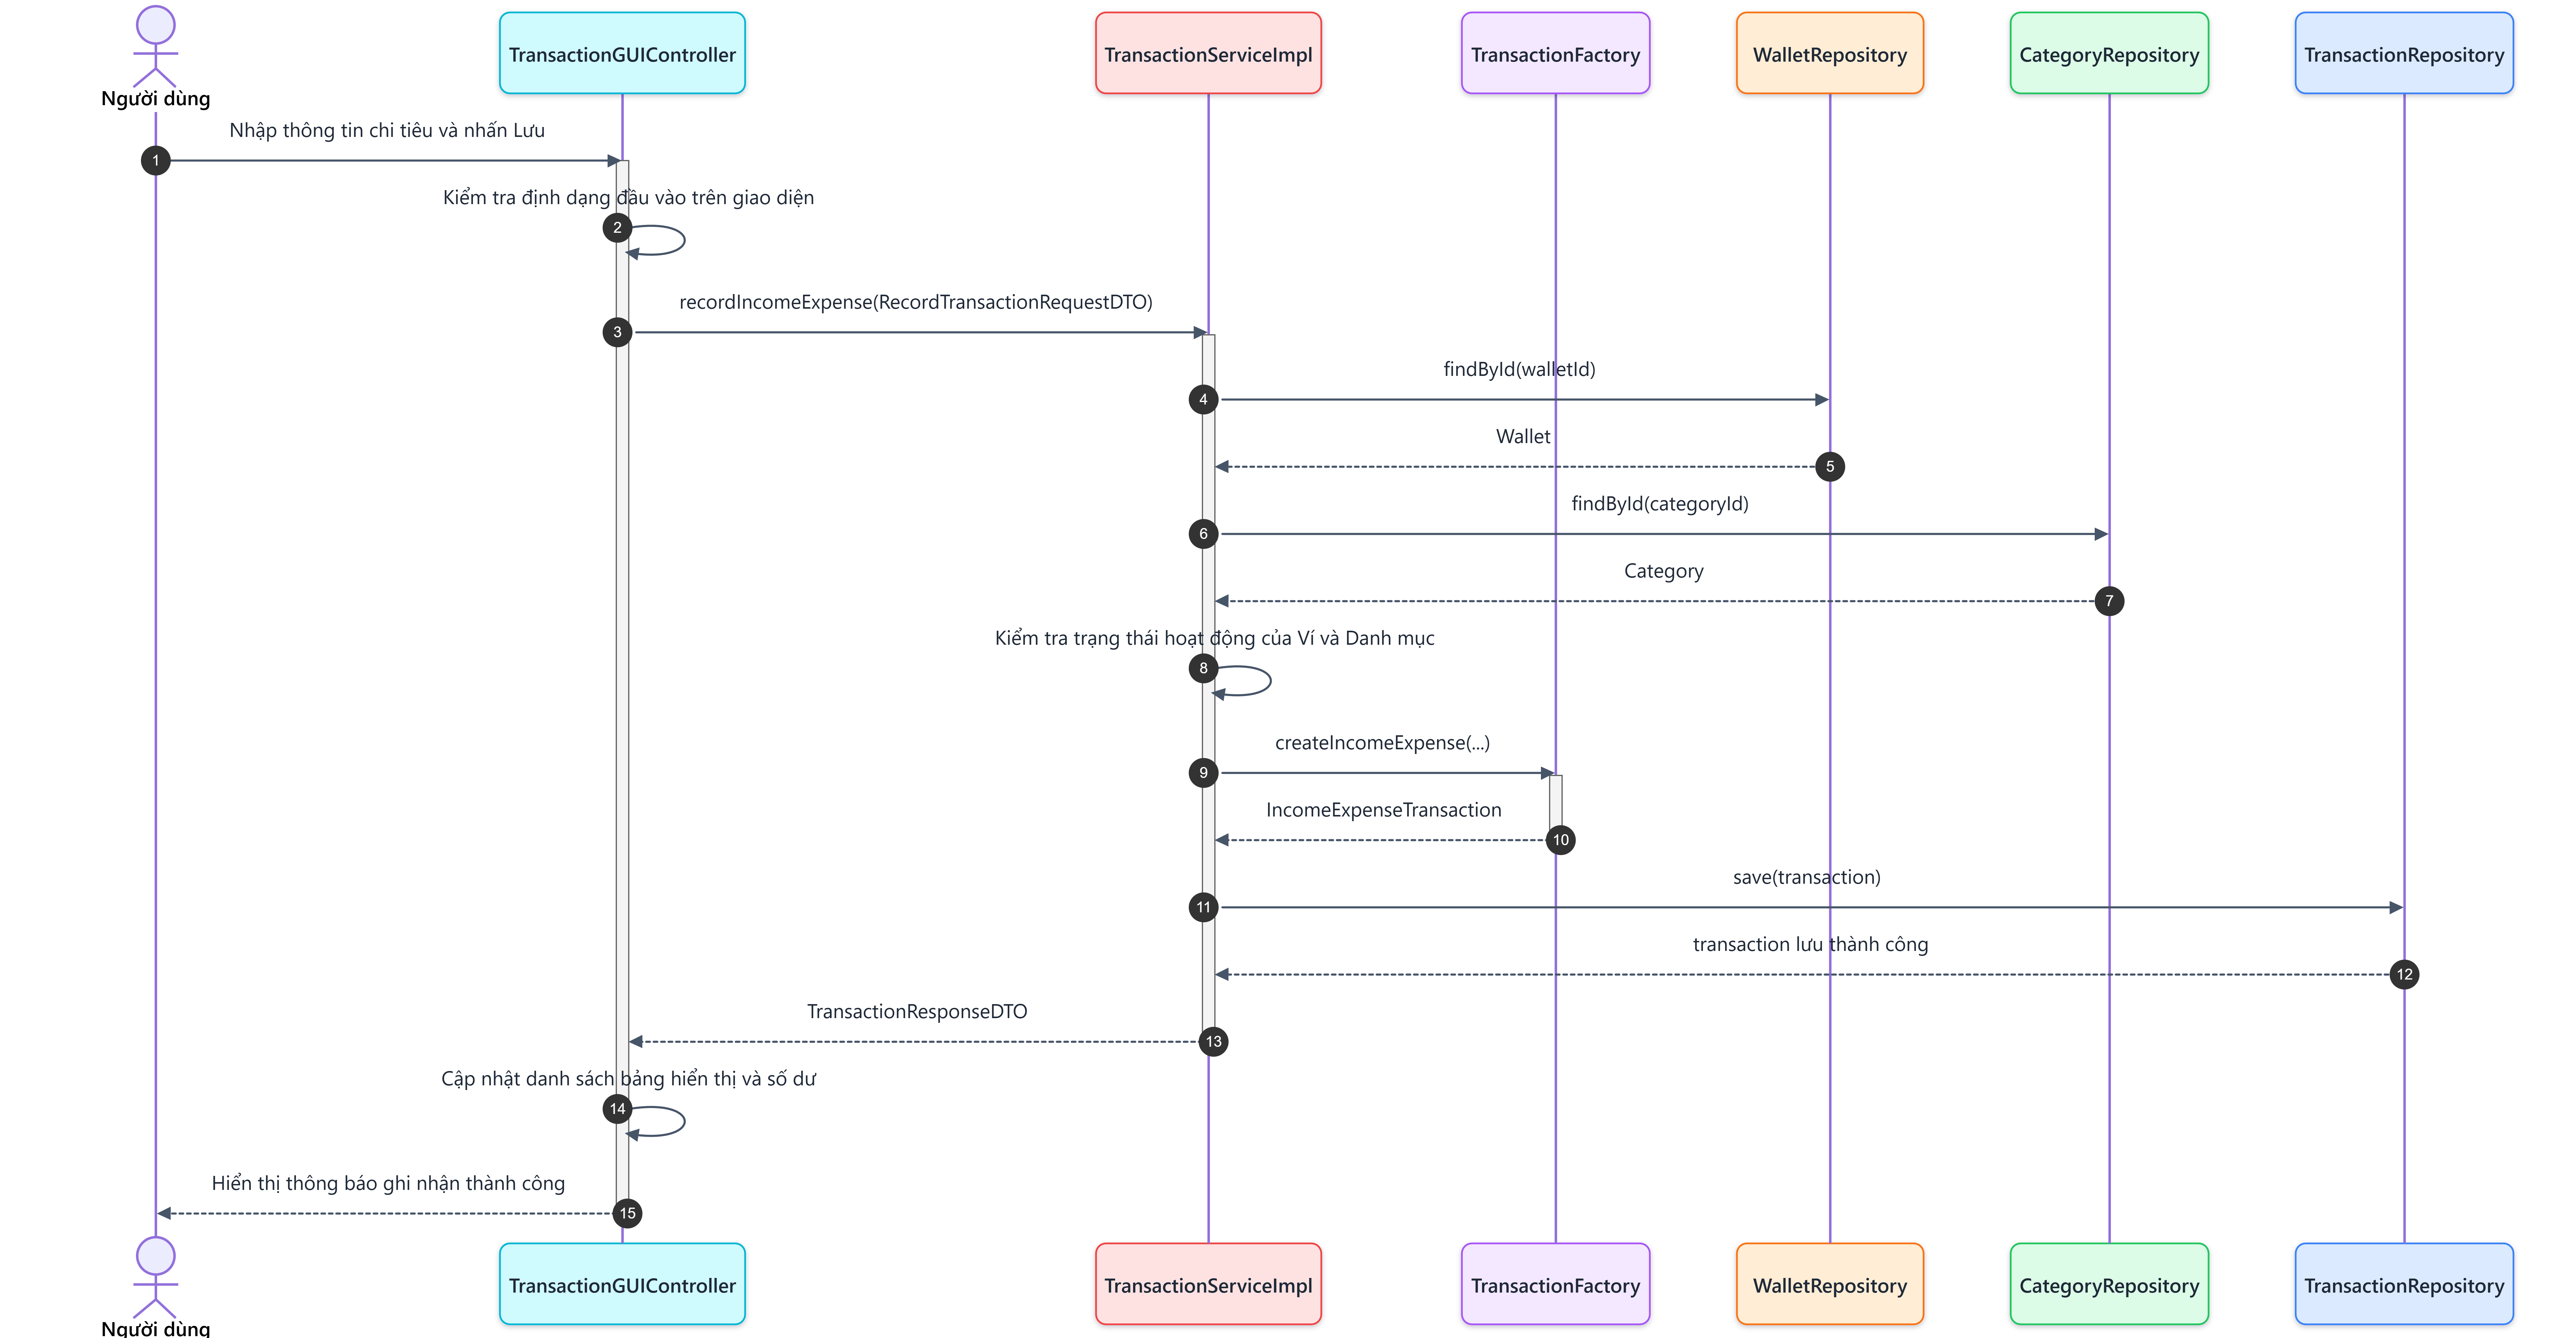
\includegraphics[width=0.85\linewidth,height=\textheight,keepaspectratio,alt={Sơ
đồ tương tác chi tiết giữa các tầng khi ghi nhận một khoản chi tiêu
mới}]{imgs/bao-cao-tong-ket-6.png}
\caption{Sơ đồ tuần tự thiết kế cho nghiệp vụ ghi nhận một khoản chi
tiêu mới}
\end{figure}

\section{Cơ chế kiểm soát lỗi và ngoại
lệ}\label{cux1a1-chux1ebf-kiux1ec3m-souxe1t-lux1ed7i-vuxe0-ngoux1ea1i-lux1ec7}

Hệ thống xây dựng một cây phân cấp ngoại lệ nghiệp vụ có cấu trúc chặt
chẽ, kế thừa trực tiếp từ lớp ngoại lệ cơ sở
\passthrough{\lstinline!BusinessException!} (thuộc nhóm
\passthrough{\lstinline!RuntimeException!}):

\begin{figure}
\centering
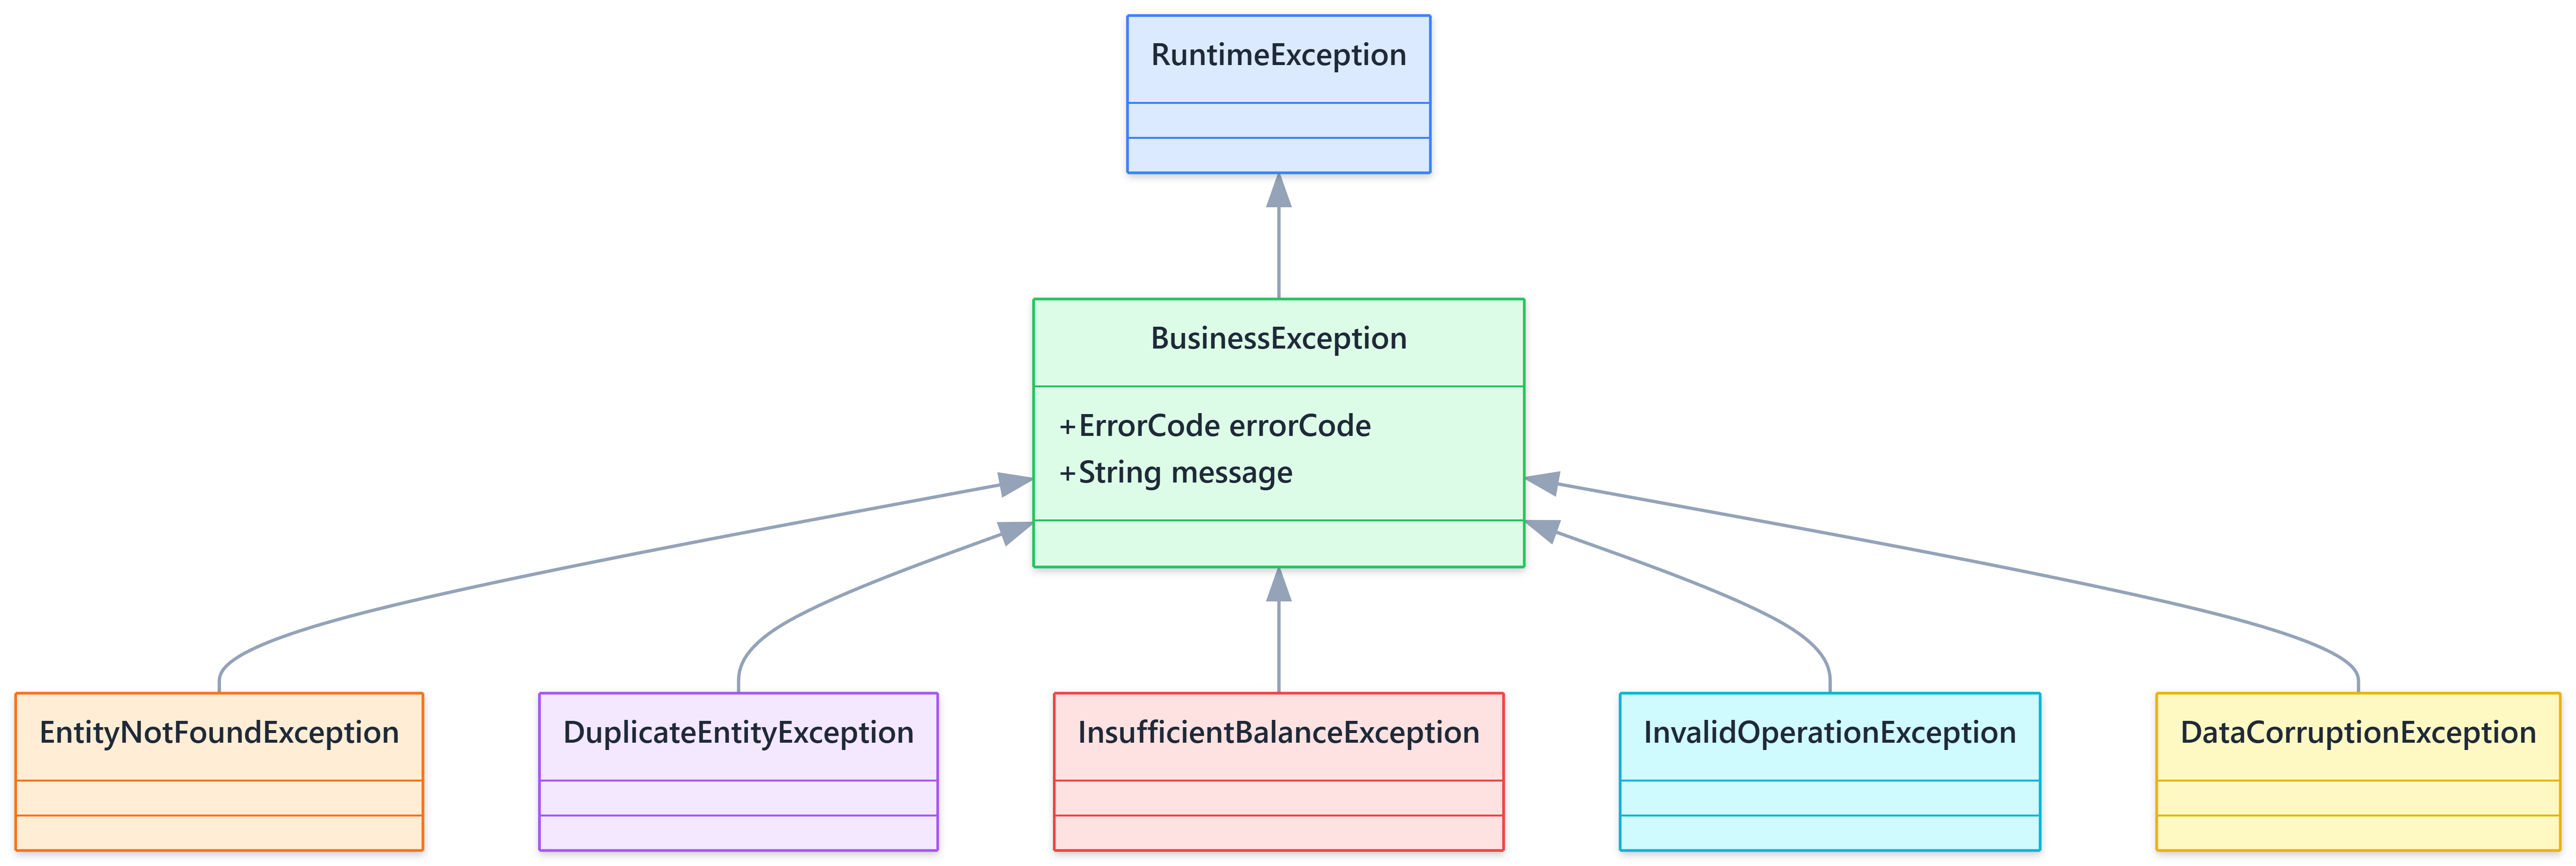
\includegraphics[width=0.85\linewidth,height=\textheight,keepaspectratio,alt={Sơ
đồ phân cấp cấu trúc kiểm soát lỗi và ngoại lệ nghiệp
vụ}]{imgs/bao-cao-tong-ket-7.png}
\caption{Sơ đồ phân cấp cấu trúc kiểm soát lỗi và ngoại lệ nghiệp vụ}
\end{figure}

Ý nghĩa và ngữ cảnh ném lỗi của từng lớp ngoại lệ: -
\passthrough{\lstinline!EntityNotFoundException!}: Ném ra khi tra cứu
một thực thể (ví, danh mục, giao dịch) theo mã định danh nhưng không tìm
thấy trong kho dữ liệu. -
\passthrough{\lstinline!DuplicateEntityException!}: Ném ra khi người
dùng cố gắng tạo ví hoặc danh mục có tên đã tồn tại trong cùng phạm vi
quản lý. - \passthrough{\lstinline!InsufficientBalanceException!}: Ném
ra khi ví nguồn không có đủ số dư khả dụng để trang trải số tiền chuyển
cùng phí phát sinh. -
\passthrough{\lstinline!InvalidOperationException!}: Ném ra khi vi phạm
các quy tắc nghiệp vụ về trạng thái, ví dụ cố gắng ghi nhận giao dịch
vào một ví đang bị đóng băng hoặc xóa một danh mục đang có giao dịch
phát sinh. - \passthrough{\lstinline!DataCorruptionException!}: Ném ra
trong quá trình đối soát dữ liệu hoặc nạp tệp sao lưu nếu phát hiện cấu
trúc tệp JSON sai lệch hoặc số liệu số dư không khớp với tổng dòng tiền
lịch sử.

Mỗi ngoại lệ đều đi kèm một mã lỗi chuẩn hóa
(\passthrough{\lstinline!ErrorCode!}) định dạng rõ ràng, cho phép tầng
trình diễn tự động chuyển dịch sang các thông điệp cảnh báo thân thiện
với người dùng cuối mà không làm lộ các chi tiết kỹ thuật nội bộ của hệ
thống.

\chapter{Cài đặt phần mềm và áp dụng mẫu thiết
kế}\label{cuxe0i-ux111ux1eb7t-phux1ea7n-mux1ec1m-vuxe0-uxe1p-dux1ee5ng-mux1eabu-thiux1ebft-kux1ebf}

\section{Áp dụng năm nguyên lý thiết kế hướng đối
tượng}\label{uxe1p-dux1ee5ng-nux103m-nguyuxean-luxfd-thiux1ebft-kux1ebf-hux1b0ux1edbng-ux111ux1ed1i-tux1b0ux1ee3ng}

Hệ thống Quản lý Tài chính Cá nhân áp dụng trọn vẹn 5 nguyên lý SOLID
trên các lớp và giao diện thực tế của dự án, bảo đảm tính gắn kết cao và
độ ghép nối lỏng:

{\def\LTcaptype{none} % do not increment counter
\begin{longtable}[]{@{}
  >{\raggedright\arraybackslash}p{(\linewidth - 4\tabcolsep) * \real{0.3333}}
  >{\raggedright\arraybackslash}p{(\linewidth - 4\tabcolsep) * \real{0.3333}}
  >{\raggedright\arraybackslash}p{(\linewidth - 4\tabcolsep) * \real{0.3333}}@{}}
\toprule\noalign{}
\begin{minipage}[b]{\linewidth}\raggedright
Nguyên lý thiết kế
\end{minipage} & \begin{minipage}[b]{\linewidth}\raggedright
Nội dung nguyên lý
\end{minipage} & \begin{minipage}[b]{\linewidth}\raggedright
Minh chứng cài đặt trong hệ thống PFMS
\end{minipage} \\
\midrule\noalign{}
\endhead
\bottomrule\noalign{}
\endlastfoot
\textbf{Đơn trách nhiệm} (SRP) & Mỗi lớp chỉ đảm nhiệm một lý do duy
nhất để thay đổi; phân định rõ giữa quy tắc nghiệp vụ, điều phối và lưu
trữ tệp. & Hệ thống phân tách độc lập giữa: thực thể
\passthrough{\lstinline!Wallet!} (chịu trách nhiệm về quy tắc và tính
toán số dư nội tại), dịch vụ \passthrough{\lstinline!WalletServiceImpl!}
(điều phối luồng ca sử dụng) và kho lưu trữ
\passthrough{\lstinline!WalletRepository!} (xử lý lưu đọc tệp). Thay đổi
về định dạng tệp JSON hoàn toàn không ảnh hưởng đến thực thể
\passthrough{\lstinline!Wallet!}. \\
\textbf{Đóng mở} (OCP) & Mở rộng cho việc bổ sung hành vi mới nhưng đóng
trước việc sửa đổi mã nguồn sẵn có. & Lớp trừu tượng
\passthrough{\lstinline!Transaction!} đóng vai trò khung cơ sở cho hai
lớp con \passthrough{\lstinline!IncomeExpenseTransaction!} và
\passthrough{\lstinline!TransferTransaction!}. Khi hệ thống cần bổ sung
loại giao dịch mới (như giao dịch đầu tư tài chính), lập trình viên chỉ
cần tạo thêm lớp con mới kế thừa \passthrough{\lstinline!Transaction!}
mà không phải sửa đổi mã nguồn lớp cha hay cấu trúc điều phối của tầng
dịch vụ. \\
\textbf{Thay thế Liskov} (LSP) & Các đối tượng lớp con có thể thay thế
hoàn toàn cho đối tượng lớp cha mà không làm sai lệch tính đúng đắn của
chương trình. & \passthrough{\lstinline!IncomeExpenseTransaction!} và
\passthrough{\lstinline!TransferTransaction!} có thể thay thế hoàn toàn
cho \passthrough{\lstinline!Transaction!} trong phương thức lưu trữ
\passthrough{\lstinline!TransactionRepository.save(Transaction)!} cũng
như trong các giải thuật trích xuất ngày và tính toán dòng tiền của
\passthrough{\lstinline!ReportServiceImpl!} mà không gây ra bất kỳ lỗi
hành vi nào. \\
\textbf{Phân tách giao diện} (ISP) & Không ép buộc các thành phần phụ
thuộc vào các giao diện chứa phương thức mà chúng không có nhu cầu sử
dụng. & Thay vì xây dựng một giao diện dịch vụ khổng lồ duy nhất, hệ
thống chia nhỏ thành 6 giao diện dịch vụ độc lập:
\passthrough{\lstinline!WalletService!},
\passthrough{\lstinline!TransactionService!},
\passthrough{\lstinline!TransferService!},
\passthrough{\lstinline!CategoryService!},
\passthrough{\lstinline!ReportService!},
\passthrough{\lstinline!DataManagementService!}. Mỗi Controller tầng
trình diễn chỉ phụ thuộc vào đúng giao diện cần dùng (ví dụ:
\passthrough{\lstinline!WalletGUIController!} chỉ phụ thuộc
\passthrough{\lstinline!WalletService!}). \\
\textbf{Nghịch đảo phụ thuộc} (DIP) & Mô đun cấp cao không phụ thuộc mô
đun cấp thấp; cả hai cùng phụ thuộc vào sự trừu tượng hóa. & Tầng dịch
vụ (\passthrough{\lstinline!WalletServiceImpl!}) không phụ thuộc trực
tiếp vào lớp đọc ghi tệp cụ thể
\passthrough{\lstinline!JsonWalletRepository!} mà phụ thuộc vào giao
diện trừu tượng \passthrough{\lstinline!WalletRepository!}. Cài đặt cụ
thể được tiêm qua hàm khởi tạo, cho phép dễ dàng hoán đổi sang
\passthrough{\lstinline!MemoryWalletRepository!} để chạy kiểm thử tự
động tốc độ cao. \\
\end{longtable}
}

Hệ thống duy trì điểm cân bằng kỹ thuật thực tế nhằm tránh thiết kế quá
mức: - Sử dụng cơ chế tiêm phụ thuộc thủ công thuần Java tại điểm khởi
động chương trình (\passthrough{\lstinline!Main!}), không đưa các khung
công nghệ nặng như Spring Framework vào ứng dụng máy tính để bàn cục bộ.
- Tái sử dụng giao diện kho lưu trữ cơ sở
\passthrough{\lstinline!GenericRepository<E, ID>!} để chuẩn hóa các thao
tác cơ bản, chỉ khai báo thêm các phương thức nghiệp vụ thực sự cần
thiết theo từng ca sử dụng.

\section{Cài đặt các mẫu thiết kế kinh
điển}\label{cuxe0i-ux111ux1eb7t-cuxe1c-mux1eabu-thiux1ebft-kux1ebf-kinh-ux111iux1ec3n}

Hệ thống chọn lọc và cài đặt 4 mẫu thiết kế hướng đối tượng cốt lõi
thuộc nhóm mẫu thiết kế kinh điển GoF nhằm chuẩn hóa quá trình tạo lập
đối tượng, đóng gói thuật toán xuất dữ liệu, quản lý trạng thái và ghi
nhận vết kiểm toán:

\subsection{Mẫu phương thức nhà máy trong khởi tạo giao
dịch}\label{mux1eabu-phux1b0ux1a1ng-thux1ee9c-nhuxe0-muxe1y-trong-khux1edfi-tux1ea1o-giao-dux1ecbch}

Lớp \passthrough{\lstinline!TransactionFactory!} được định vị tại tầng
nghiệp vụ (\passthrough{\lstinline!com.pfms.domain.model!}) nhằm đóng
gói toàn bộ quy trình tiếp nhận tham số, phân định đa hình và khởi tạo
đúng loại giao dịch:

\begin{figure}
\centering
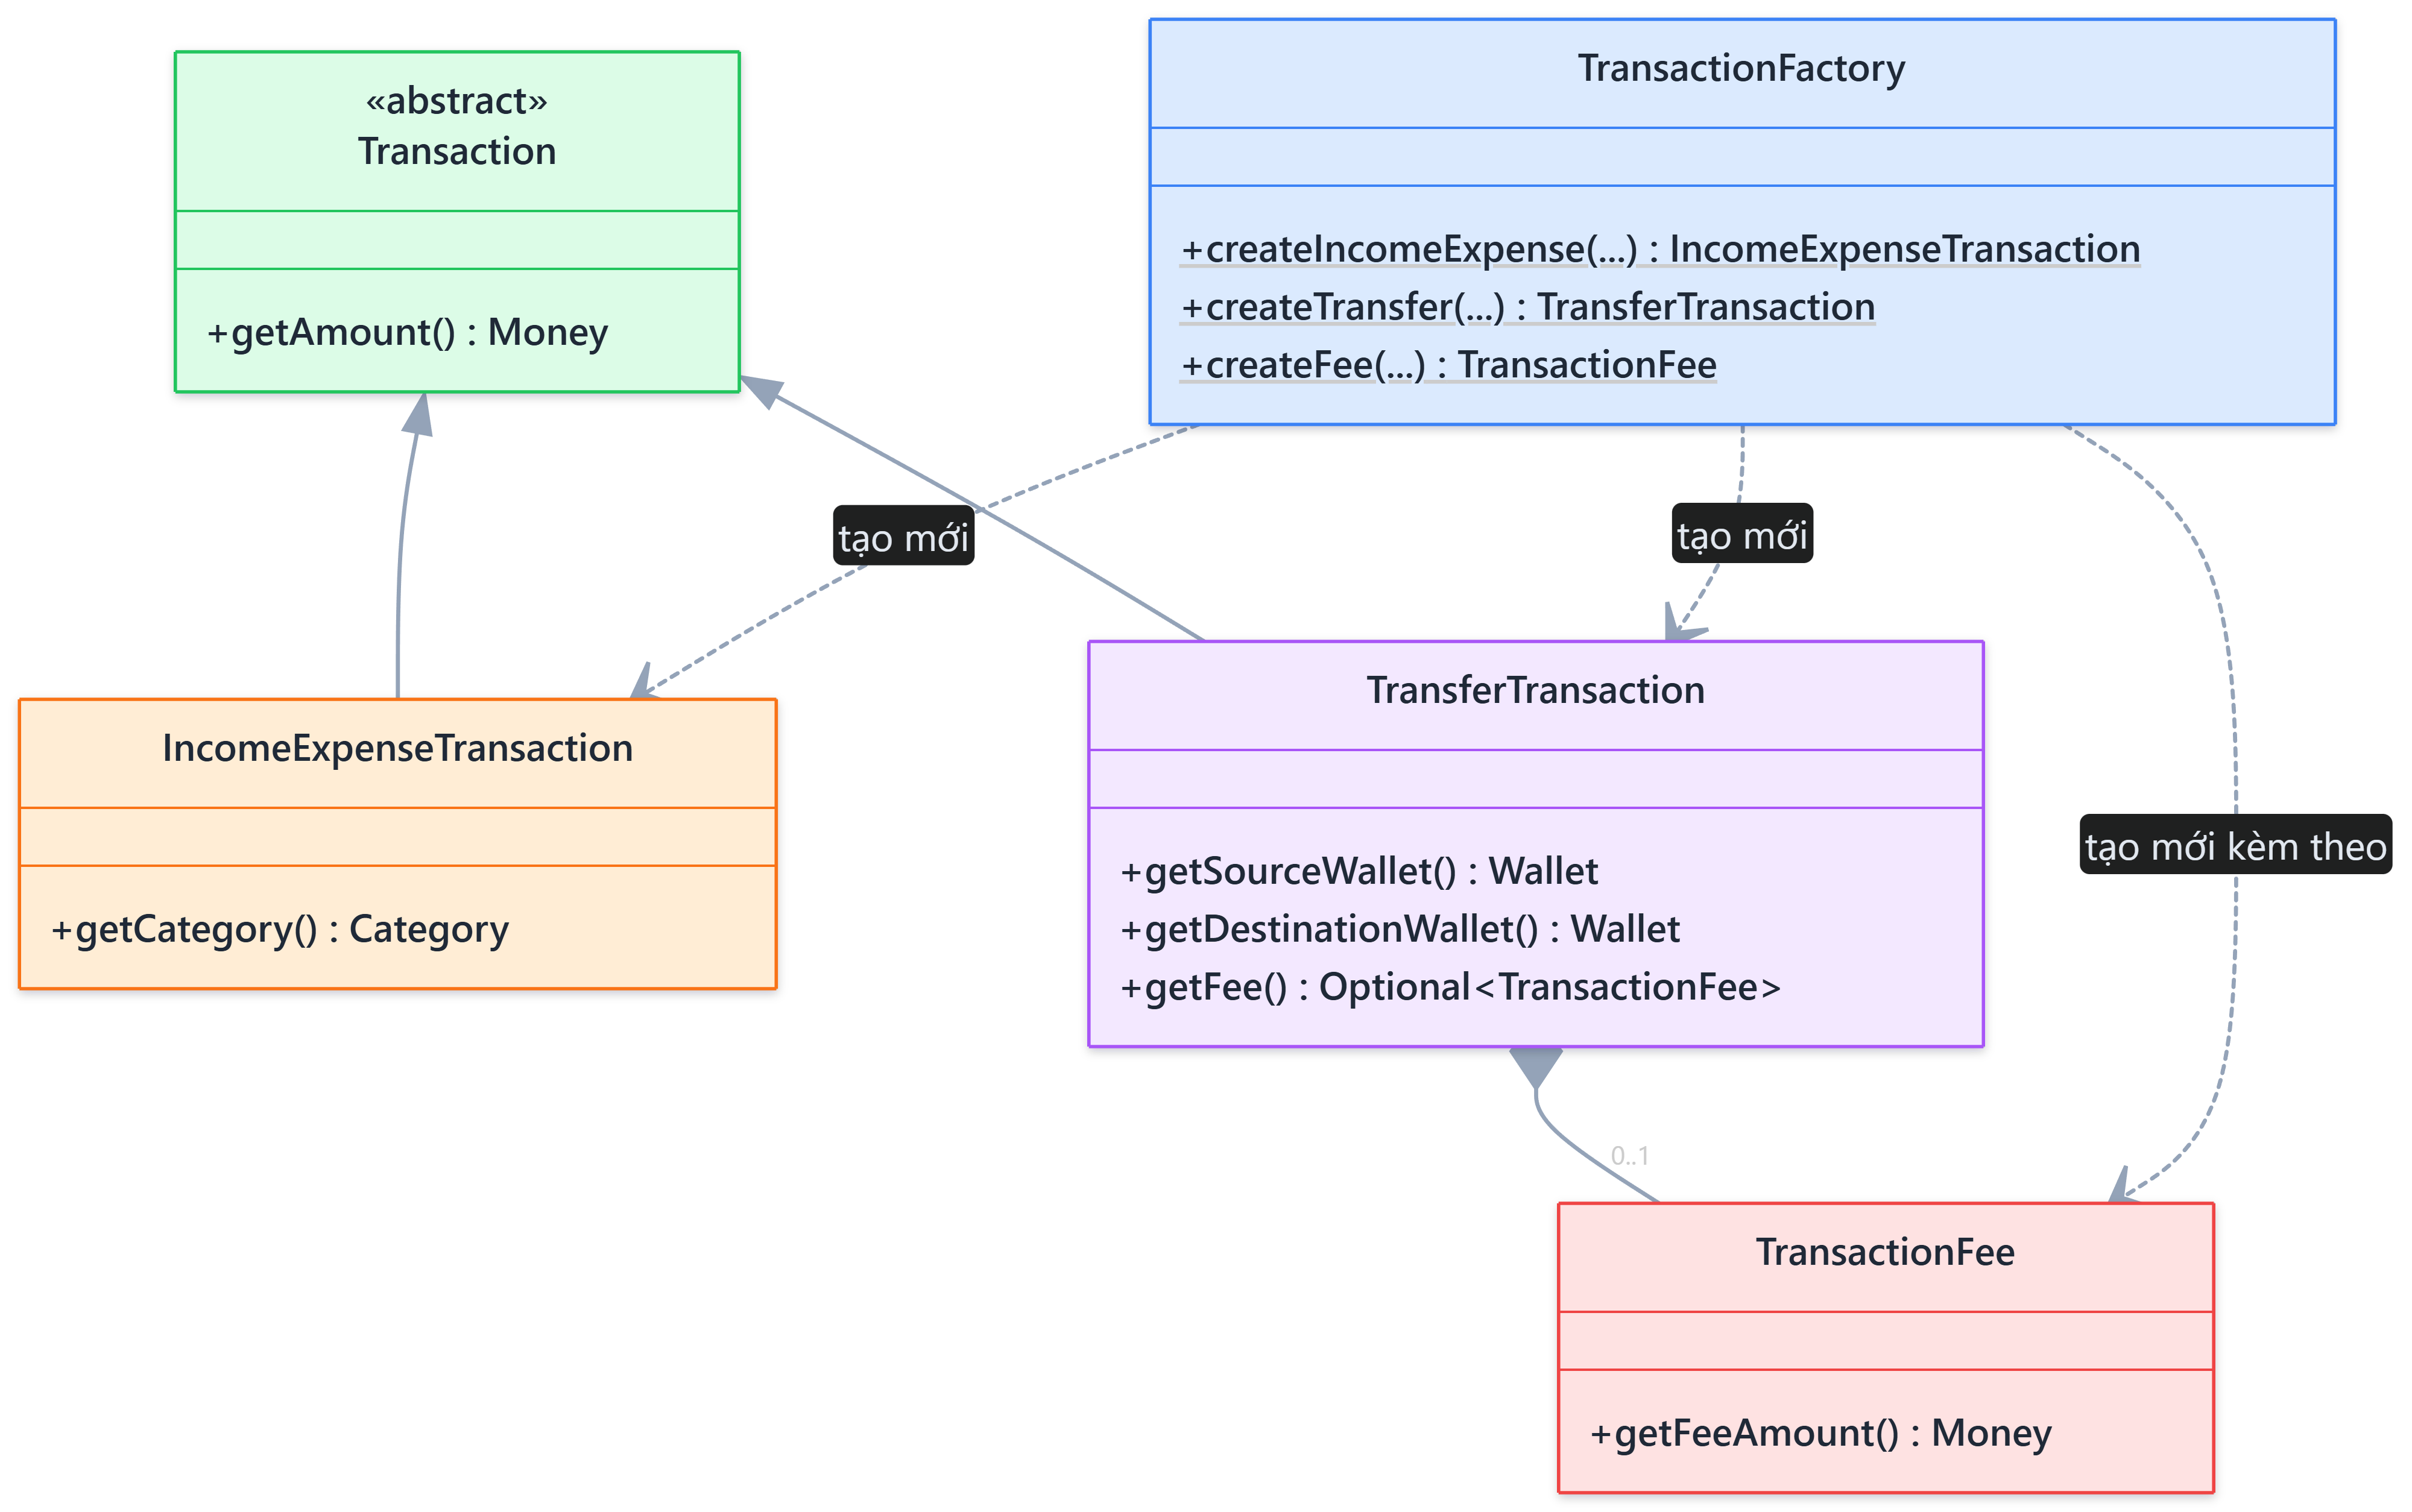
\includegraphics[width=0.85\linewidth,height=\textheight,keepaspectratio,alt={Cài
đặt mẫu phương thức nhà máy (Factory Method Pattern) trong khởi tạo giao
dịch}]{imgs/bao-cao-tong-ket-8.png}
\caption{Cài đặt mẫu phương thức nhà máy (Factory Method Pattern) trong
khởi tạo giao dịch}
\end{figure}

Lợi ích kỹ thuật: - Đóng gói trọn vẹn quy trình tạo lập giao dịch phức
tạp kèm chi phí hợp thành sinh tử. - Giải phóng các lớp dịch vụ
\passthrough{\lstinline!TransactionServiceImpl!} và
\passthrough{\lstinline!TransferServiceImpl!} khỏi việc gọi trực tiếp
lệnh \passthrough{\lstinline!new!} cho từng lớp con, giúp tầng dịch vụ
không bị phụ thuộc vào chi tiết cài đặt của các lớp cụ thể.

\subsection{Mẫu chiến lược trong xuất báo cáo tài
chính}\label{mux1eabu-chiux1ebfn-lux1b0ux1ee3c-trong-xuux1ea5t-buxe1o-cuxe1o-tuxe0i-chuxednh}

Hệ thống sử dụng mẫu thiết kế Chiến lược để đóng gói các thuật toán định
dạng và xuất báo cáo tài chính ra nhiều định dạng khác nhau:

\begin{figure}
\centering
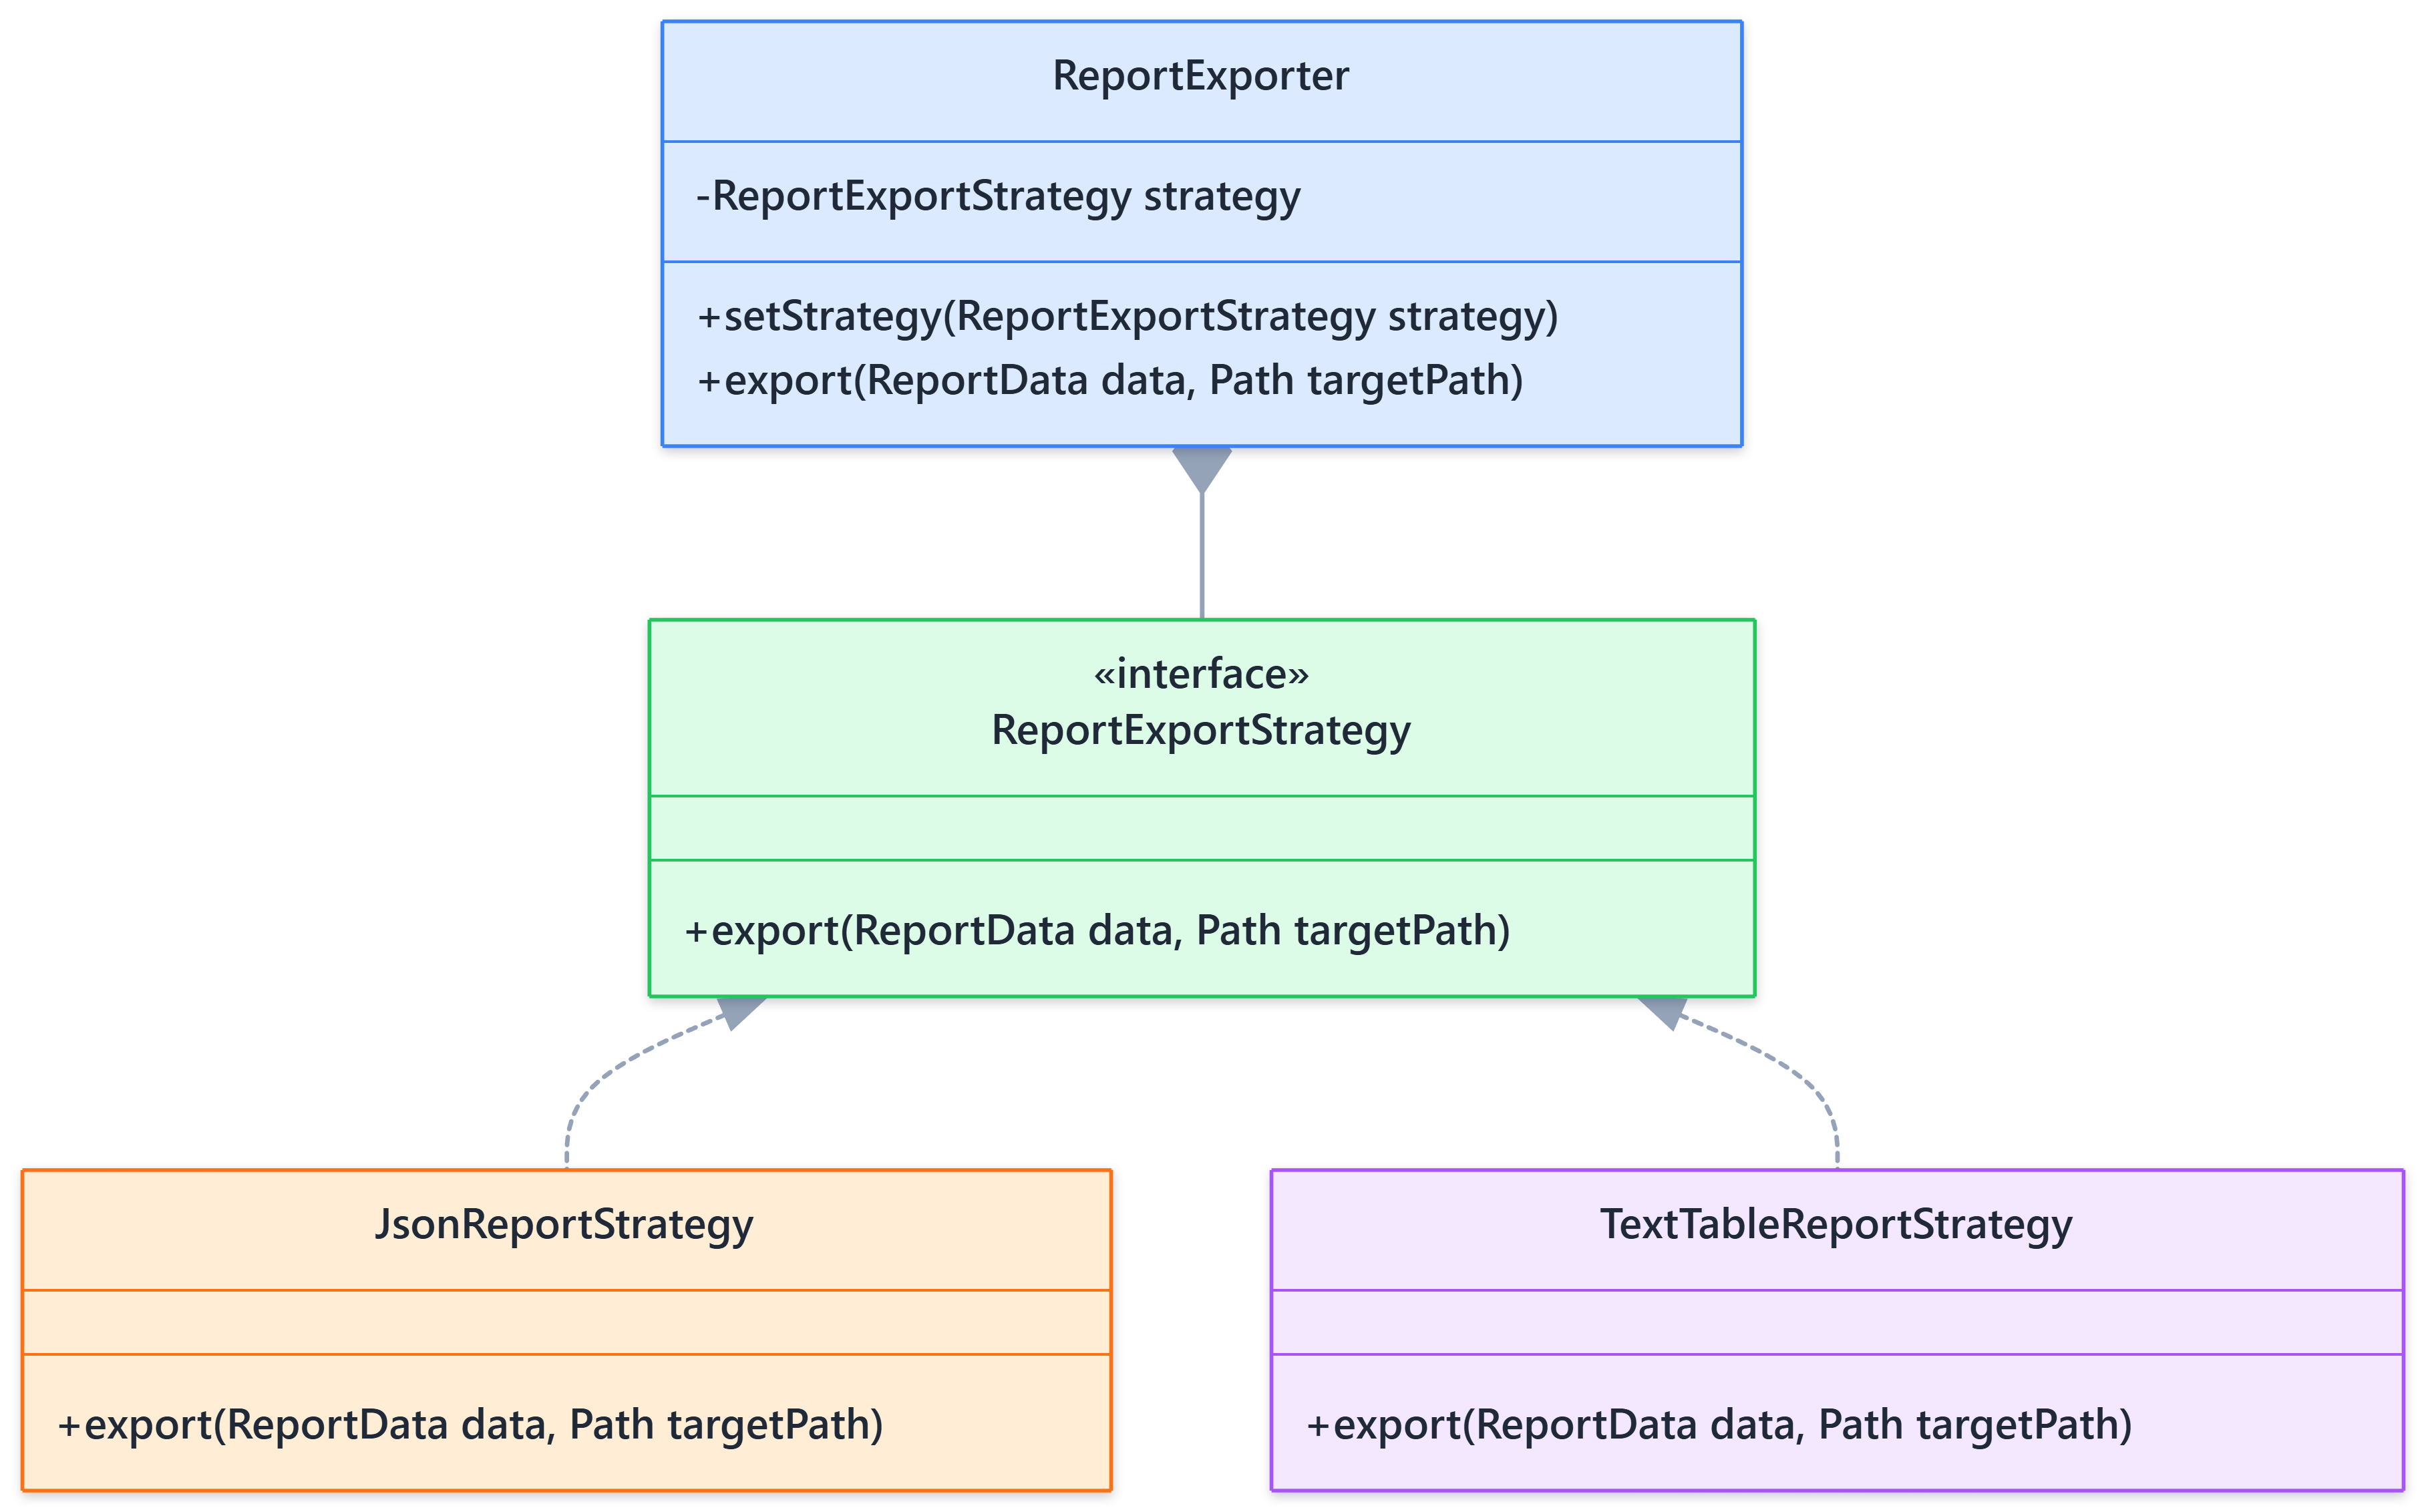
\includegraphics[width=0.85\linewidth,height=\textheight,keepaspectratio,alt={Cài
đặt mẫu chiến lược (Strategy Pattern) trong xuất báo cáo tài
chính}]{imgs/bao-cao-tong-ket-9.png}
\caption{Cài đặt mẫu chiến lược (Strategy Pattern) trong xuất báo cáo
tài chính}
\end{figure}

Lợi ích kỹ thuật: - Giao diện
\passthrough{\lstinline!ReportExportStrategy!} định nghĩa phương thức
xuất dữ liệu chuẩn mực
\passthrough{\lstinline!export(ReportData data, Path targetPath)!}. -
Hai chiến lược cài đặt gồm \passthrough{\lstinline!JsonReportStrategy!}
(kết xuất tệp cấu trúc JSON phục vụ lưu trữ trao đổi) và
\passthrough{\lstinline!TextTableReportStrategy!} (kết xuất báo cáo bảng
văn bản định dạng bảng ASCII phục vụ in ấn hoặc đọc nhanh). - Lớp ngữ
cảnh \passthrough{\lstinline!ReportExporter!} cho phép tráo đổi linh
hoạt định dạng xuất tại thời điểm thực thi dựa trên lựa chọn của người
dùng tại giao diện mà không phải sửa đổi mã nguồn điều phối.

\subsection{Mẫu trạng thái trong quản lý vòng đời thực
thể}\label{mux1eabu-trux1ea1ng-thuxe1i-trong-quux1ea3n-luxfd-vuxf2ng-ux111ux1eddi-thux1ef1c-thux1ec3}

Thực thể Ví tiền (\passthrough{\lstinline!Wallet!}) đóng vai trò ngữ
cảnh áp dụng mẫu thiết kế Trạng thái để kiểm soát vòng đời và hành vi
biến động số dư. Cấu trúc lớp gồm giao diện
\passthrough{\lstinline!WalletState!} và 3 lớp trạng thái cụ thể: -
\passthrough{\lstinline!ActiveWalletState!}: Trạng thái hoạt động, tiếp
nhận bình thường mọi biến động dòng tiền gồm nạp tiền
(\passthrough{\lstinline!credit!}), chi tiêu
(\passthrough{\lstinline!debit!}), chuyển tiền và cho phép chuyển sang
trạng thái lưu trữ hoặc xóa. -
\passthrough{\lstinline!ArchivedWalletState!}: Trạng thái lưu trữ, số dư
vẫn được tính vào tổng tài sản nhưng từ chối mọi giao dịch thu chi hoặc
điều chuyển tiền mới. Trạng thái này chỉ cho phép thao tác kích hoạt lại
(\passthrough{\lstinline!activate!}). -
\passthrough{\lstinline!DeletedWalletState!}: Trạng thái đã xóa, từ chối
mọi biến động số dư và thao tác chuyển đổi trạng thái.

Việc đóng gói hành vi vào các lớp trạng thái giúp loại bỏ hoàn toàn các
khối lệnh rẽ nhánh điều kiện lặp lại \passthrough{\lstinline!if-else!}
trong các phương thức của \passthrough{\lstinline!Wallet!}.

\subsection{Mẫu người quan sát trong theo dõi biến động dữ
liệu}\label{mux1eabu-ngux1b0ux1eddi-quan-suxe1t-trong-theo-duxf5i-biux1ebfn-ux111ux1ed9ng-dux1eef-liux1ec7u}

Hệ thống áp dụng mẫu thiết kế Người quan sát để xử lý các tác vụ phụ trợ
sau khi một giao dịch tài chính hoàn tất mà không làm thắt chặt khớp nối
trong tầng dịch vụ: - Nguồn phát sự kiện: Lớp
\passthrough{\lstinline!TransactionServiceImpl!} phối hợp cùng bộ điều
phối \passthrough{\lstinline!TransactionEventPublisher!} đóng vai trò là
chủ thể phát sự kiện. - Giao diện người quan sát: Giao diện
\passthrough{\lstinline!TransactionEventListener!} định nghĩa phương
thức tiếp nhận sự kiện
\passthrough{\lstinline!onTransactionCreated(TransactionCreatedEvent event)!}.
- Các bộ lắng nghe cụ thể:
\passthrough{\lstinline!WalletBalanceUpdateListener!} (cập nhật số dư
tức thời lên ví liên quan theo quy tắc bảo toàn) và
\passthrough{\lstinline!AuditLogEventListener!} (ghi nhận vết kiểm toán
vào nhật ký hệ thống phục vụ đối soát). - Đối tượng sự kiện:
\passthrough{\lstinline!TransactionCreatedEvent!} đóng gói bất biến
thông tin mã giao dịch, số tiền và mốc thời gian.

Cơ chế này giúp tầng dịch vụ chỉ tập trung vào việc hạch toán giao dịch
chính mà không bị phụ thuộc vào các phân hệ ghi nhật ký hay kiểm toán
bên ngoài.

\section{Xử lý tính toán tài chính chính xác và cấu trúc dữ
liệu}\label{xux1eed-luxfd-tuxednh-touxe1n-tuxe0i-chuxednh-chuxednh-xuxe1c-vuxe0-cux1ea5u-truxfac-dux1eef-liux1ec7u}

Trong lập trình tài chính, độ chính xác số học là yếu tố sống còn. Hệ
thống thiết lập các chuẩn mực kỹ thuật nghiêm ngặt trong mã nguồn:

\begin{enumerate}
\def\labelenumi{\arabic{enumi}.}
\item
  Xử lý số học tài chính chuẩn mực với
  \passthrough{\lstinline!BigDecimal!}: Toàn bộ các phép tính tiền tệ
  trong lớp \passthrough{\lstinline!Money!} và các lớp dịch vụ đều sử
  dụng \passthrough{\lstinline!BigDecimal!} được khởi tạo từ chuỗi ký tự
  (\passthrough{\lstinline!String!}) hoặc số nguyên, tuyệt đối không
  khởi tạo từ số thực \passthrough{\lstinline!double!} để tránh sai số
  biểu diễn nhị phân. Các phép toán chia tỷ lệ và tính tỷ trọng đều chỉ
  định rõ thang đo 4 chữ số thập phân và áp dụng quy tắc làm tròn nửa
  chẵn (\passthrough{\lstinline!RoundingMode.HALF\_EVEN!}), triệt tiêu
  hoàn toàn sai số làm tròn tích lũy.
\item
  Bảo vệ cấu trúc dữ liệu với Collections không thể sửa đổi: Khi các
  thực thể hoặc lớp dịch vụ trả về danh sách tập hợp các giao dịch hoặc
  danh mục, hệ thống luôn bọc kết quả thông qua
  \passthrough{\lstinline!Collections.unmodifiableList(...)!} hoặc sao
  chép phòng thủ. Kỹ thuật này ngăn chặn các thành phần bên ngoài can
  thiệp làm biến đổi trực tiếp danh sách dữ liệu nội bộ của thực thể,
  bảo vệ tính toàn vẹn của mô hình hướng đối tượng.
\item
  Kiểm tra tiền điều kiện với lớp tiện ích
  \passthrough{\lstinline!Preconditions!}: Hệ thống xây dựng lớp tiện
  ích tập trung \passthrough{\lstinline!Preconditions!} để thẩm định dữ
  liệu đầu vào ngay tại cửa ngõ của các hàm khởi tạo và phương thức dịch
  vụ:
\end{enumerate}

\begin{itemize}
\tightlist
\item
  \passthrough{\lstinline!requireNonBlank(String text, String message)!}:
  Đảm bảo chuỗi ký tự không rỗng và không chỉ chứa khoảng trắng.
\item
  \passthrough{\lstinline!requirePositive(BigDecimal amount, String message)!}:
  Đảm bảo số tiền phát sinh phải lớn hơn 0.
\item
  \passthrough{\lstinline!requireNonNegative(BigDecimal amount, String message)!}:
  Đảm bảo số dư ban đầu không được âm.
\item
  \passthrough{\lstinline!requireValidDateRange(LocalDate from, LocalDate to)!}:
  Đảm bảo ngày bắt đầu không được sau ngày kết thúc. Các kiểm tra này
  giúp hệ thống phát hiện và ngăn chặn dữ liệu không hợp lệ từ sớm
  (Fail-fast principle).
\end{itemize}

\chapter{Kiểm thử, vận hành và đánh giá kết
quả}\label{kiux1ec3m-thux1eed-vux1eadn-huxe0nh-vuxe0-ux111uxe1nh-giuxe1-kux1ebft-quux1ea3}

\section{Chiến lược kiểm thử tự
động}\label{chiux1ebfn-lux1b0ux1ee3c-kiux1ec3m-thux1eed-tux1ef1-ux111ux1ed9ng}

Hệ thống Quản lý Tài chính Cá nhân áp dụng chiến lược kiểm thử tự động
toàn diện với khung kiểm thử JUnit 5, kết hợp chặt chẽ với phương pháp
phát triển hướng kiểm thử TDD:

\begin{enumerate}
\def\labelenumi{\arabic{enumi}.}
\item
  Kiểm thử đơn vị cô lập: Mọi thực thể nghiệp vụ và đối tượng giá trị
  đều được bao phủ bởi các bài kiểm thử đơn vị độc lập. Lớp
  \passthrough{\lstinline!MoneyTest!} kiểm tra toàn diện các phép toán
  cộng, trừ, nhân tỷ lệ, làm tròn nửa chẵn và so sánh tiền tệ. Lớp
  \passthrough{\lstinline!WalletTest!} kiểm tra việc khởi tạo, bảo toàn
  số dư và tính toán số dư mới khi có biến động.
\item
  Kiểm thử giá trị biên và ràng buộc dữ liệu: Hệ thống thiết kế các ca
  kiểm thử chuyên biệt để rà soát hành vi tại các điểm giới hạn: số tiền
  giao dịch bằng 0, số tiền giao dịch cực đại (lên đến hàng trăm tỷ đồng
  mà không bị tràn số), độ dài tên ví và tên danh mục tại đúng các mốc
  biên 1 ký tự và 50 ký tự, chuỗi ký tự chứa khoảng trắng hoặc ký tự đặc
  biệt.
\item
  Kiểm thử chuyển trạng thái thực thể: Các bài kiểm thử trạng thái thẩm
  định việc chuyển đổi giữa các trạng thái
  \passthrough{\lstinline!ACTIVE!}, \passthrough{\lstinline!ARCHIVED!}
  và \passthrough{\lstinline!DELETED!}, bảo đảm hệ thống từ chối các
  thao tác sai ngữ cảnh (ví dụ: không cho phép ghi nhận giao dịch vào ví
  đã lưu trữ hoặc không cho phép xóa danh mục khi đang có giao dịch tham
  chiếu).
\item
  Kiểm thử tầng dịch vụ độc lập với bộ nhớ tạm: Bằng cách sử dụng các
  kho lưu trữ trong bộ nhớ
  (\passthrough{\lstinline!MemoryWalletRepository!},
  \passthrough{\lstinline!MemoryTransactionRepository!}\ldots), toàn bộ
  các ca sử dụng phức tạp của tầng dịch vụ được kiểm thử với đầy đủ các
  kịch bản thành công và ngoại lệ mà không phải phụ thuộc vào việc đọc
  ghi tệp vật lý trên đĩa.
\end{enumerate}

\section{Kết quả kiểm thử thực tế trên hệ
thống}\label{kux1ebft-quux1ea3-kiux1ec3m-thux1eed-thux1ef1c-tux1ebf-truxean-hux1ec7-thux1ed1ng}

Quá trình xây dựng và kiểm thử hệ thống được tự động hóa hoàn toàn thông
qua công cụ Apache Maven. Kết quả thực thi thực tế của bộ kiểm thử trên
toàn bộ dự án:

\begin{lstlisting}
-------------------------------------------------------
 T E S T S
-------------------------------------------------------
Results:

Tests run: 2288, Failures: 0, Errors: 0, Skipped: 0

------------------------------------------------------------------------
BUILD SUCCESS
------------------------------------------------------------------------
Total time:  18.062 s
\end{lstlisting}

Bảng phân bổ các ca kiểm thử theo từng phân hệ kiến trúc:

{\def\LTcaptype{none} % do not increment counter
\begin{longtable}[]{@{}
  >{\raggedright\arraybackslash}p{(\linewidth - 6\tabcolsep) * \real{0.2500}}
  >{\raggedright\arraybackslash}p{(\linewidth - 6\tabcolsep) * \real{0.2500}}
  >{\raggedright\arraybackslash}p{(\linewidth - 6\tabcolsep) * \real{0.2500}}
  >{\raggedright\arraybackslash}p{(\linewidth - 6\tabcolsep) * \real{0.2500}}@{}}
\toprule\noalign{}
\begin{minipage}[b]{\linewidth}\raggedright
Phân hệ mã nguồn
\end{minipage} & \begin{minipage}[b]{\linewidth}\raggedright
Số lượng ca kiểm thử
\end{minipage} & \begin{minipage}[b]{\linewidth}\raggedright
Tỷ lệ thành công
\end{minipage} & \begin{minipage}[b]{\linewidth}\raggedright
Trọng tâm kiểm thử
\end{minipage} \\
\midrule\noalign{}
\endhead
\bottomrule\noalign{}
\endlastfoot
\textbf{Thực thể và Đối tượng giá trị}
(\passthrough{\lstinline!domain.model!}) & 522 tests & 100\% (522/522) &
Độ chính xác số học \passthrough{\lstinline!Money!}, tính bất biến, quy
tắc nghiệp vụ nội tại của \passthrough{\lstinline!Wallet!},
\passthrough{\lstinline!Transaction!},
\passthrough{\lstinline!Category!}. \\
\textbf{Ngoại lệ và Tiện ích}
(\passthrough{\lstinline!domain.exception!},
\passthrough{\lstinline!common.util!}) & 121 tests & 100\% (121/121) &
Các điều kiện ném lỗi của \passthrough{\lstinline!Preconditions!}, ánh
xạ mã lỗi và kiểm tra định dạng dữ liệu. \\
\textbf{Tầng Dịch vụ ứng dụng} (\passthrough{\lstinline!service.impl!})
& 360 tests & 100\% (360/360) & Điều phối nghiệp vụ, chuyển tiền nguyên
tử hai pha, tính toán báo cáo dòng tiền, kiểm kê số dư và kiểm tra ràng
buộc toàn vẹn. \\
\textbf{Tầng Hạ tầng lưu trữ} (\passthrough{\lstinline!infrastructure!})
& 218 tests & 100\% (218/218) & Cơ chế đọc ghi tệp JSON, an toàn tệp qua
cơ chế ghi nguyên tử, đối soát tệp sao lưu. \\
\textbf{Tầng Trình diễn và Điều khiển}
(\passthrough{\lstinline!presentation!}) & 1.067 tests & 100\%
(1067/1067) & Khởi tạo giao diện đồ họa Swing, kiểm tra biến đổi DTO, bộ
điều khiển sự kiện và các chiến lược xuất báo cáo. \\
\textbf{Tổng cộng toàn hệ thống} & \textbf{2.288 tests} & \textbf{100\%}
& \textbf{Hệ thống đạt trạng thái không lỗi (0 failures, 0 errors, 0
skipped).} \\
\end{longtable}
}

\section{Giao diện ứng dụng và kịch bản vận
hành}\label{giao-diux1ec7n-ux1ee9ng-dux1ee5ng-vuxe0-kux1ecbch-bux1ea3n-vux1eadn-huxe0nh}

Hệ thống xây dựng giao diện đồ họa người dùng bằng Java Swing, tuân thủ
mô hình kiến trúc Model-View-Presenter (MVP) và tổ chức mã nguồn theo
tính năng (Package-by-Feature):

Cấu trúc giao diện người dùng: - Màn hình Tổng quan Ví: Bảng thống kê
danh sách ví tài khoản, hiển thị số dư tính lại từ dòng tiền lịch sử,
nút tạo ví mới, cập nhật ví và hộp thoại kiểm kê điều chỉnh số dư. - Màn
hình Ghi nhận Giao dịch: Form nhập liệu thu chi với danh mục thả xuống
theo nhóm nhu cầu, bảng lịch sử giao dịch hỗ trợ lọc tức thời theo ví,
khoảng thời gian và từ khóa. - Màn hình Chuyển tiền nội bộ: Form điều
chuyển tiền giữa hai ví, tính năng tính phí chuyển tiền tùy chọn, bảng
lịch sử chuyển tiền và nút hoàn tác giao dịch. - Màn hình Quản lý Danh
mục: Cây danh mục 3 cấp trực quan cho phép thêm mới danh mục con, đổi
tên danh mục và xóa an toàn có cảnh báo ràng buộc dữ liệu. - Màn hình
Báo cáo và Thống kê: Bảng tổng hợp dòng tiền thuần 12 tháng, cơ cấu chi
tiêu theo nhóm nhu cầu và nút xuất báo cáo ra tệp JSON hoặc bảng văn bản
in ấn. - Màn hình Quản trị Dữ liệu: Tính năng xuất bản sao lưu hệ thống
ra tệp JSON, nạp phục hồi từ bản sao lưu và nút bấm kiểm tra đối soát
toàn vẹn số học.

Kịch bản vận hành trình diễn hệ thống qua 6 bước: 1. Bước 1: Khởi động
ứng dụng từ màn hình chính. Người dùng kiểm tra ví mặc định ``Tiền mặt''
(khởi điểm 0 VND) và tạo thêm ``Ví Ngân hàng''. Người dùng ghi nhận
khoản thu nhập đầu kỳ 5.000.000 VND vào ví tiền mặt và 10.000.000 VND
vào ví ngân hàng để hình thành số dư hoạt động ban đầu theo đúng quy tắc
bảo toàn số dư. 2. Bước 2: Truy cập phân hệ Danh mục, kiểm tra các danh
mục chuẩn đã được nạp sẵn. Người dùng tạo thêm danh mục con ``Cà phê
sáng'' thuộc nhóm ``Nhu cầu linh hoạt''. 3. Bước 3: Truy cập phân hệ
Giao dịch, ghi nhận một khoản chi tiêu 45.000 VND cho danh mục ``Cà phê
sáng'' từ ``Ví Tiền mặt''. Hệ thống ghi nhận thành công, số dư ``Ví Tiền
mặt'' tự động cập nhật về 4.955.000 VND. 4. Bước 4: Truy cập phân hệ
Chuyển tiền, thực hiện chuyển 2.000.000 VND từ ``Ví Ngân hàng'' sang
``Ví Tiền mặt'' với chi phí chuyển tiền là 1.100 VND. Hệ thống khấu trừ
2.001.100 VND tại ví ngân hàng và cộng đúng 2.000.000 VND vào ví tiền
mặt. 5. Bước 5: Truy cập phân hệ Báo cáo, xem biểu bảng dòng tiền và cơ
cấu chi tiêu trong tháng hiện tại. Người dùng nhấn nút xuất báo cáo ra
tệp bảng văn bản để lưu trữ. 6. Bước 6: Truy cập phân hệ Quản trị dữ
liệu, xuất toàn bộ dữ liệu ra tệp sao lưu JSON an toàn và chạy chức năng
đối soát số học. Hệ thống thông báo toàn bộ dữ liệu được bảo toàn nguyên
vẹn với 0 sai lệch.

\section{Đánh giá kết quả đạt được và hướng phát
triển}\label{ux111uxe1nh-giuxe1-kux1ebft-quux1ea3-ux111ux1ea1t-ux111ux1b0ux1ee3c-vuxe0-hux1b0ux1edbng-phuxe1t-triux1ec3n}

Đánh giá kết quả đạt được: - Hệ thống hoàn thành 100\% mục tiêu ban đầu
của đề tài môn học, đáp ứng đầy đủ 20 ca sử dụng chuẩn hóa trải đều trên
6 phân hệ nghiệp vụ. - Thiết kế hướng đối tượng chặt chẽ, tuân thủ xuất
sắc 5 nguyên lý SOLID và áp dụng hiệu quả 4 mẫu thiết kế GoF kinh điển.
- Toàn bộ các phép tính tiền tệ được bảo vệ bằng kiểu dữ liệu có độ
chính xác cao \passthrough{\lstinline!BigDecimal!} và quy tắc làm tròn
nửa chẵn, triệt tiêu hoàn toàn sai số tích lũy. - Chất lượng phần mềm
được kiểm chứng định lượng bằng 2.288 bài kiểm thử tự động với tỷ lệ
vượt qua tuyệt đối 100\%.

Giới hạn kỹ thuật hiện tại: - Ứng dụng vận hành dưới dạng phần mềm máy
tính để bàn cục bộ đơn người dùng, chưa hỗ trợ đồng bộ hóa dữ liệu trực
tuyến qua mạng giữa nhiều thiết bị khác nhau. - Cơ chế lưu trữ sử dụng
tệp JSON phẳng, phù hợp tối ưu cho dữ liệu cá nhân (dưới 100.000 bản
ghi) nhưng chưa khai thác các hệ quản trị cơ sở dữ liệu quan hệ cho các
bài toán quy mô lớn.

Hướng phát triển trong tương lai: - Bổ sung biểu đồ trực quan động và
nâng cao trải nghiệm người dùng với các giao diện hiện đại hơn. - Mở
rộng hỗ trợ tính năng quản lý danh mục đầu tư tài chính sinh lời và đa
tiền tệ với bảng tỷ giá quy đổi linh hoạt. - Đóng gói ứng dụng thành tệp
cài đặt độc lập cho từng hệ điều hành máy trạm.

\chapter{Tài liệu tham khảo}\label{tuxe0i-liux1ec7u-tham-khux1ea3o}

\begin{enumerate}
\def\labelenumi{\arabic{enumi}.}
\tightlist
\item
  Bloch, J. (2018). \emph{Effective Java} (3rd ed.). Addison-Wesley
  Professional.
\item
  Cockburn, A. (2001). \emph{Writing Effective Use Cases}.
  Addison-Wesley Professional.
\item
  Evans, E. (2003). \emph{Domain-Driven Design: Tackling Complexity in
  the Heart of Software}. Addison-Wesley.
\item
  Fowler, M. (2002). \emph{Patterns of Enterprise Application
  Architecture}. Addison-Wesley Professional.
\item
  Gamma, E., Helm, R., Johnson, R., \& Vlissides, J. (1994).
  \emph{Design Patterns: Elements of Reusable Object-Oriented Software}.
  Addison-Wesley.
\item
  IEEE/ISO/IEC. (2018). \emph{ISO/IEC/IEEE 29148:2018 Systems and
  software engineering: Life cycle processes: Requirements engineering}.
  IEEE.
\item
  Larman, C. (2004). \emph{Applying UML and Patterns: An Introduction to
  Object-Oriented Analysis and Design and Iterative Development} (3rd
  ed.). Prentice Hall.
\item
  Martin, R. C. (2018). \emph{Clean Architecture: A Craftsman's Guide to
  Software Structure and Design}. Prentice Hall.
\end{enumerate}

\end{document}
